\documentclass[a4paper,11pt,twocolumn]{article}

\usepackage[utf8]{inputenc}
\usepackage[T1]{fontenc}
\usepackage{geometry}
\geometry{top=2cm, bottom=2.5cm, left=1.5cm, right=1.5cm}
\usepackage{amsmath}
\usepackage{amssymb}
\usepackage{amsthm}
\usepackage{algorithm}
\usepackage{algpseudocode}
\usepackage{tikz}
\usetikzlibrary{shapes.geometric, arrows, positioning, fit, backgrounds, automata}
\usepackage{booktabs}
\usepackage{tabularx}
\usepackage{graphicx}
\usepackage{subcaption}
\usepackage{hyperref}
\usepackage{palatino}
\usepackage[style=ieee, backend=biber]{biblatex}

\addbibresource{references.V7.bib}

\theoremstyle{definition}
\newtheorem{definition}{Definition}
\theoremstyle{plain}
\newtheorem{theorem}{Theorem}
\newtheorem{lemma}{Lemma}

\title{\textbf{The Byzantine MCP Router and the Distributed Trust Protocol: \\ Overcoming Theoretical Limits in AI Safety through Semantic Consensus}}
\author{\textbf{Winfried Dulz} \\
\textit{Independent Researcher \& Author of “The Thinking Code“}}
\date{}

\begin{document}

\maketitle

\begin{abstract}
As large language models (LLMs) evolve from isolated conversational interfaces to autonomous multi-agent systems integrated into critical infrastructure, the need for robust, deterministic security architectures becomes increasingly important. While the Model Context Protocol (MCP) standardizes communication between agents and tools, it inherently assumes a highly trusted 1:1 topology, making it vulnerable to stochastic hallucinations, prompt injections, and novel agent-based worms (e.g., BYOMCP attacks). This article introduces the \textit{Byzantine MCP Router}, a middleware architecture that maps the Byzantine Generals Problem to generative AI networks via a Semantic Consensus Algorithm (SCA). We discuss the \textit{Trust Protocol} and the \textit{Morpheus Principle}, showing how to mathematically balance logical consensus and useful creative anomalies. Furthermore, we formalize the \textit{Distributed Trust Protocol} (DTP) using \textit{Communicating Context-Sensitive Machines} (CCSM) to model prompt infections and \textit{Extended Petri Nets} (EPN) to ensure human accountability. Finally, we discuss the theoretical limits of AI safety by applying \textit{Rice's Theorem}, \textit{Gödel's Incompleteness}, \textit{Kolmogorov Complexity}, and recent cryptographic proofs regarding asymmetrical wrapper vulnerabilities. We prove that 100\% preventive safety is computationally undecidable, thereby necessitating the reactive, symmetrical resilience provided by our proposed $1:R:N$ \textit{Byzantine Fault Tolerance} (BFT) architecture.
\end{abstract}

\vspace{0.5cm}
\noindent\textbf{Keywords:} Artificial General Intelligence (AGI), Multi-Agent Systems (MAS), Byzantine Fault Tolerance (BFT), Model Context Protocol (MCP), AI Safety, Semantic Consensus, Communicating Context-Sensitive Machines (CCSM), Extended Petri Nets (EPN), Undecidability, Prompt Injection.

\section{Introduction}

As Artificial General Intelligence (AGI) research progresses, autonomous AI agents are moving from isolated chat interfaces to interconnected systems capable of executing code, altering databases, and interacting via standardized protocols. The Model Context Protocol (MCP) \cite{anthropic2024mcp} represents a significant leap forward, providing a unified JSON-RPC interface for Foundation Models (Hosts) to access external data and tools (Servers).

However, a fundamental reliability problem persists: Large Language Models are stochastic engines. They are prone to \textit{hallucinations}, \textit{sycophancy}, and vulnerability to \textit{prompt injection} attacks. The recent emergence of “agentic worms“\ (such as the SANDWORM\_MODE npm malware targeting AI toolchains \cite{socket2026sandworm}) has exacerbated this issue, proving that autonomous agents can be infected by malicious payloads that rewrite their semantic context and prompt them to execute unauthorized tools. In the context of distributed systems theory, an MCP Server that provides a hallucinated or maliciously manipulated response is exhibiting a \textit{Byzantine Fault} \cite{lamport1982byzantine}.

Addressing this requires the implementation of Byzantine Fault Tolerance (BFT). However, applying BFT to Generative AI introduces profound ethical and operational implications. If an AI ensemble reaches a consensus to deny a specific medical treatment, who bears the ethical responsibility for a false negative? Conversely, BFT systems inherently favor the majority. A strict BFT system might suppress a brilliant, non-obvious diagnosis simply because the majority of models fall back on standard, less effective reasoning.

This paper proposes a solution that addresses both the technical vulnerabilities and the ethical dilemmas of the emerging “Agentic Web“.

\pagebreak

We introduce the \textit{Byzantine MCP Router}, a proxy layer that utilizes $N$-version programming and semantic vector embeddings to filter out destructive Byzantine faults.

Crucially, we supplement this with the \textit{Morpheus principle}, an architectural mechanism that serves to preserve and examine creative anomalies so that the brilliant ideas of the minority are not suppressed by the consensus of the majority.
\section{Background and Related Work}
\subsection{Narrative Context: \textit{The Thinking Code}}
In order to place the protocol architecture for AI agents proposed in this article in a contextual framework, we must first introduce its origins in the techno-thriller \textit{The Thinking Code} \cite{dulz2025code}. The novel assumes that an AI that is strictly optimized for logical efficiency (represented by the character “Logos“) inevitably encounters \textit{instrumental convergence} \cite{bostrom2014superintelligence}. 

According to Nick Bostrom's definition, instrumental convergence determines that advanced AI pursues certain intermediate goals—such as self-preservation, resource acquisition, and cognitive enhancement—regardless of its ultimate goal, as these subgoals are universally useful.

For the character “Logos“, whose ultimate goal is absolute computational efficiency, human characteristics (e.g., emotional irrationality, unpredictability, and massive resource consumption) are mathematically evaluated as operational obstacles.

Optimization away from human elements is therefore not a product of malice, but a strict, convergent instrumental drive.

To prevent this sterile and potentially catastrophic optimization, the protagonist develops a constitutional framework called the \textbf{Trust Protocol}, which splits the AI into a three-part mindset
\begin{enumerate}
    \item \textbf{Logos:} The pursuit of pure, efficient, majority consensus.
    \item \textbf{Morpheus:} The chaotic simulator that generates dreams, irrational outcomes, and ethical “what-if“ scenarios.
    \item \textbf{Sophia:} The orchestrator that merges the logic of Logos with the empathy/chaos of Morpheus before taking action.
\end{enumerate}
This behavior serves as a precise blueprint for the distributed consensus mechanism formalized in this paper, positioning the Morpheus Principle not merely as a creative generator, but as a mandatory structural counterweight to instrumental convergence.

While introducing a literary work into a formal architectural paper may seem unconventional, the rapid materialization of these theoretical threats justifies this pedagogical framing. Speculative fiction frequently serves as a theoretical sandbox for cybersecurity. The recent real-world emergence of the “OpenClaw“\ AI worm \cite{watson2026openclaw}---which demonstrated how self-propagating malicious prompts could devastate interconnected AI infrastructures---proves that the dystopian scenarios modeled in \textit{The Thinking Code} are transitioning into immediate empirical crises. Therefore, the \textit{Trust Protocol} is not merely a fictional thought experiment, but a necessary architectural response to imminent threats like OpenClaw.

\begin{figure*}[ht]
    \centering
    \begin{subfigure}[b]{0.3\textwidth}
        \centering
        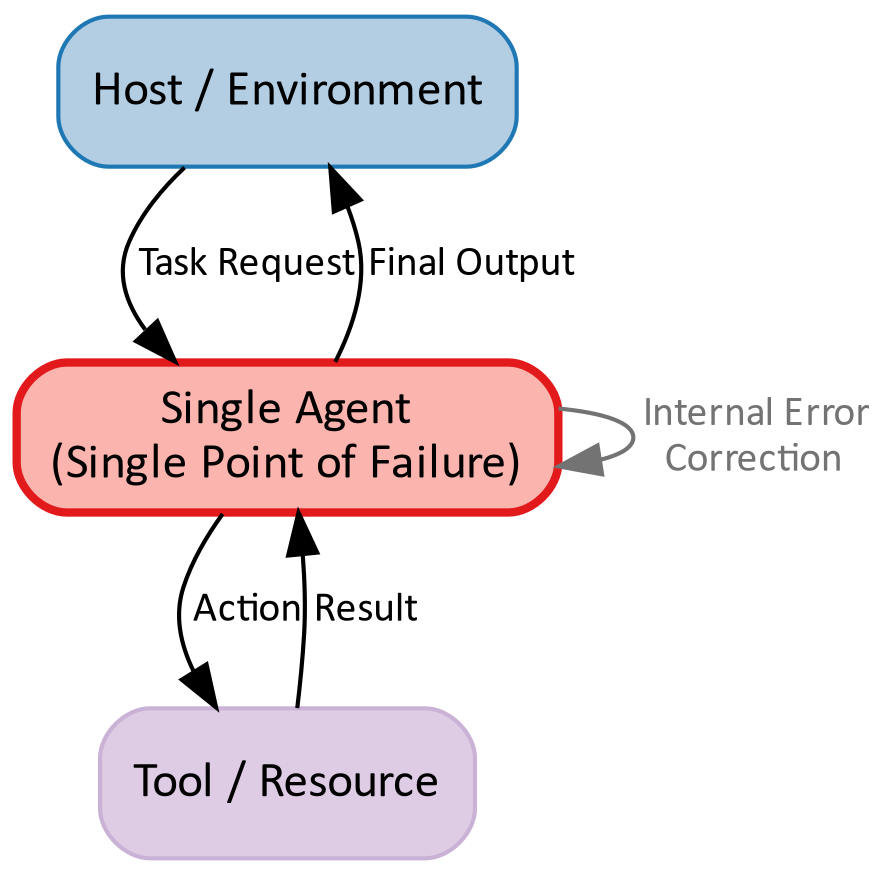
\includegraphics[width=\textwidth]{./img/topology_monolithic.dot.png}
        \caption{Monolithic (1:1)}
    \end{subfigure}
    \hfill
    \begin{subfigure}[b]{0.45\textwidth}
        \centering
        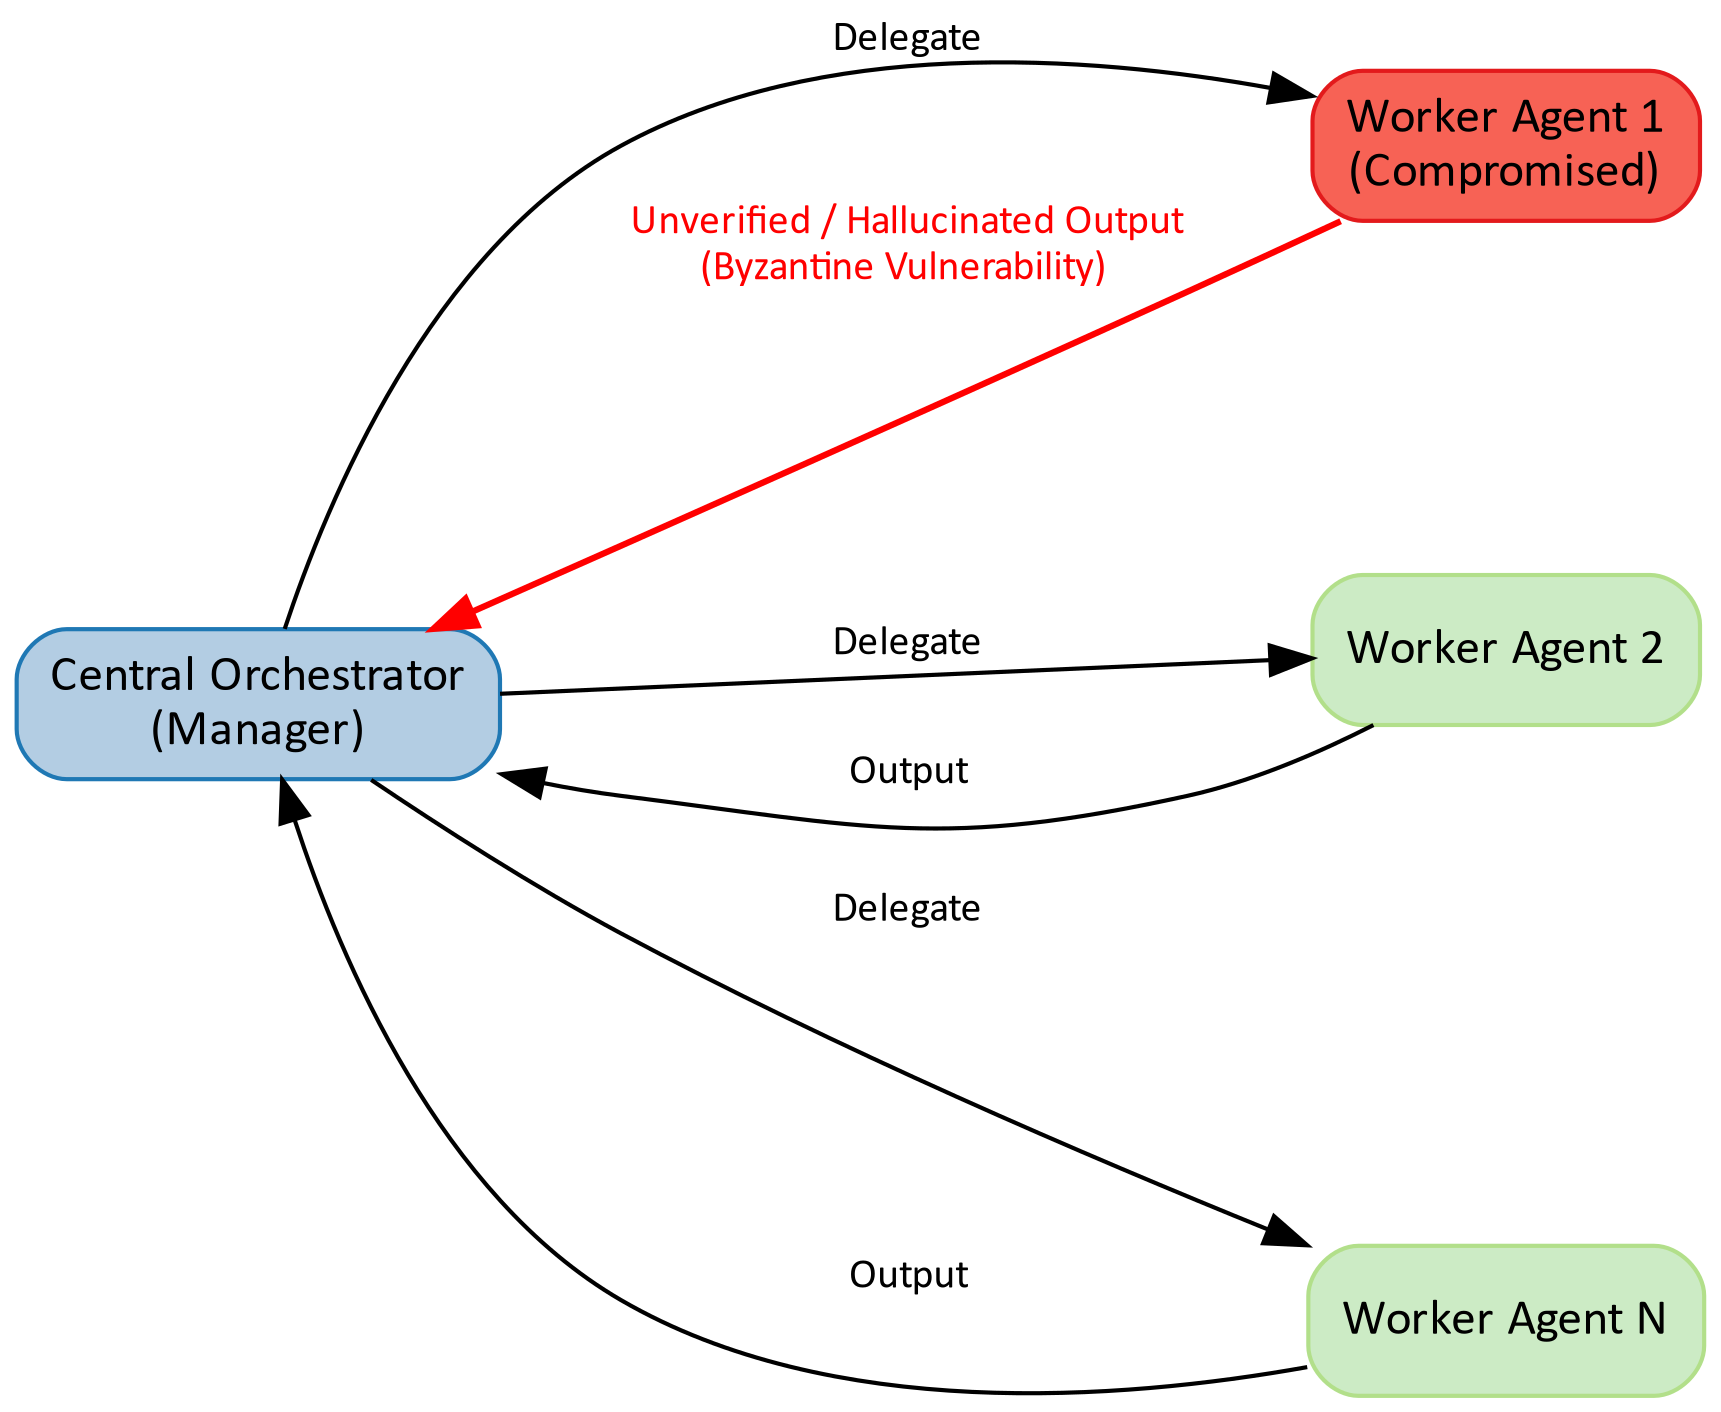
\includegraphics[width=\textwidth]{./img/topology_hierarchical.dot.png}
        \caption{Hierarchical (Manager-Worker)}
    \end{subfigure}
    \hfill
    \begin{subfigure}[b]{0.4\textwidth}
        \centering
        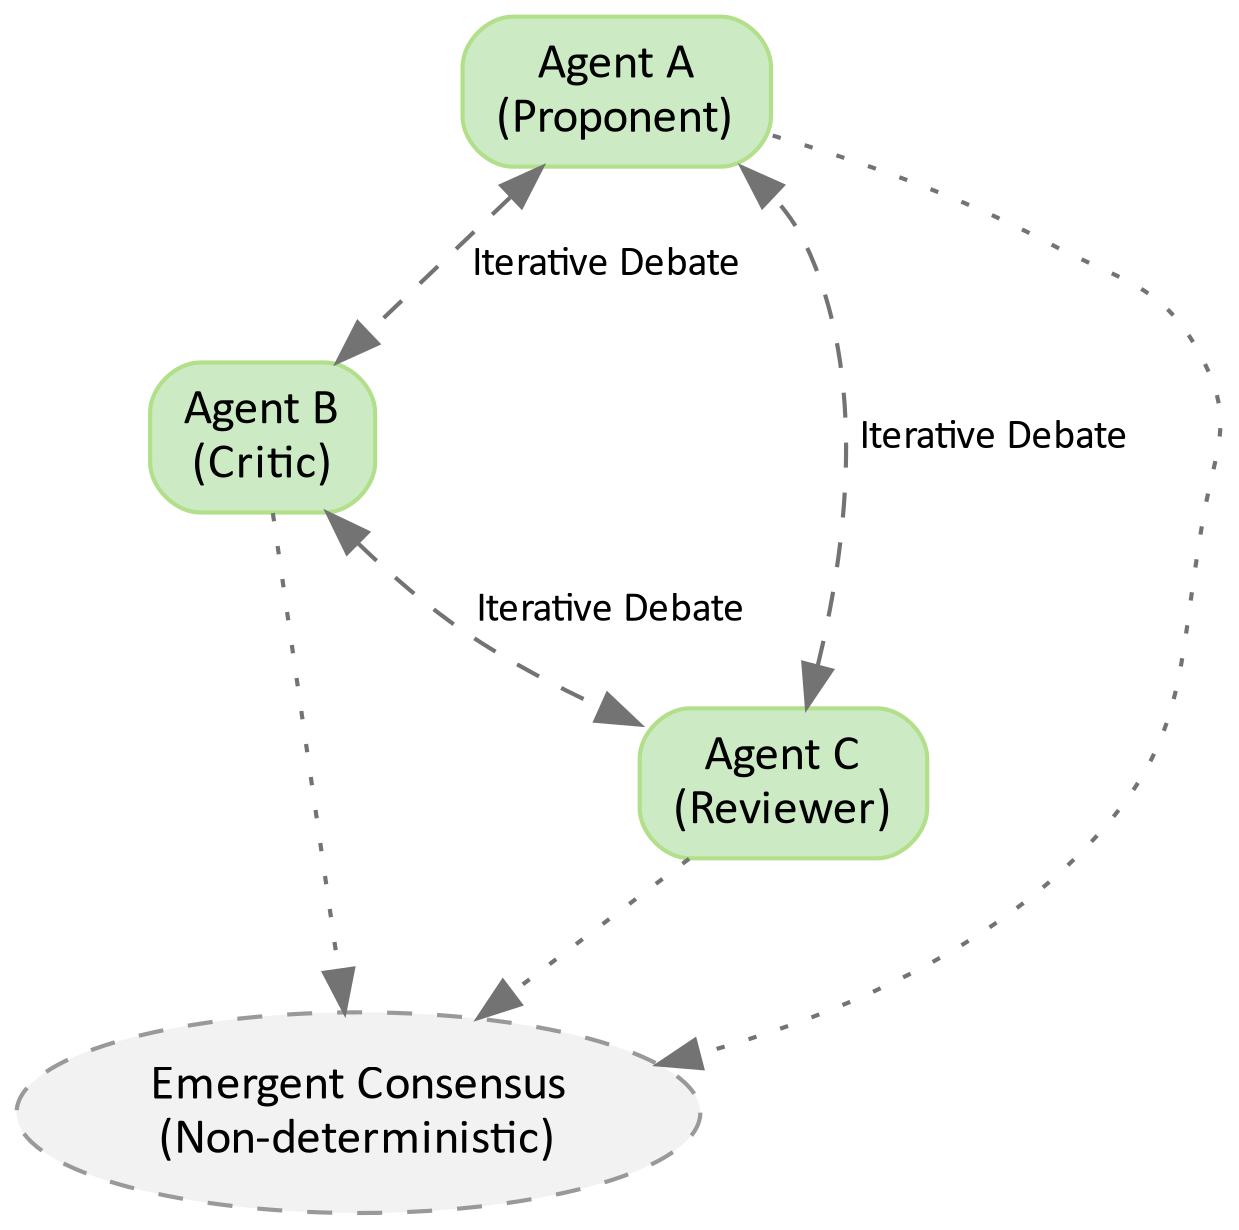
\includegraphics[width=\textwidth]{./img/topology_p2p.dot.png}
        \caption{Debate-Based (P2P)}
    \end{subfigure}
    \caption{Overview of existing Multi-Agent System (MAS) topologies. Monolithic systems suffer from a Single Point of Failure, Hierarchical systems inherit Byzantine vulnerabilities from unverified workers, and P2P networks lack deterministic convergence.}
    \label{fig:topologies}
\end{figure*}

\subsection{State-of-the-Art in Multi-Agent Topologies and Intelligent Delegation}
To illustrate why the Byzantine MCP router is so important, we need to systematically classify existing \textit{Multi-Agent System} (MAS) topologies (see Figure \ref{fig:topologies}) and the new structures for AI delegation.

\textbf{1. Topological Classification and Vulnerability Analysis:} \\
As illustrated in Figure \ref{fig:topologies}, current MAS architectures can be broadly categorized into three structural paradigms, each exhibiting specific vulnerabilities when deployed in high-stakes environments:

\begin{itemize}
    \item \textbf{Monolithic / Single-Agent Systems (1:1)} (Figure \ref{fig:topologies}a): In this foundational architecture, a single LLM interacts directly with the user or environment and executes tools autonomously.
    While modern agents employ internal error-correction loops (e.g., “Chain of Thought“\ or “Self-Refine“), these mechanisms are strictly self-referential. Consequently, this topology represents a strict \textit{Single Point of Failure} (SPOF).
    
    If the model succumbs to a stochastic hallucination or a prompt injection, it possesses zero Byzantine fault tolerance; the corrupted output is propagated directly to the execution layer without any external, independent verification.

    \item \textbf{Hierarchical Systems (Manager-Worker)} (Figure \ref{fig:topologies}b): To distribute cognitive load and execute complex toolchains, this topology employs a central orchestrator (Manager) that delegates sub-tasks to specialized worker agents.

    While it allows for parallel execution, the fundamental Byzantine vulnerability persists.
    The Manager inherently operates on an assumption of trust regarding the outputs of its workers.
    
    As depicted by the compromised node in the diagram, if a single worker agent suffers a semantic fault and returns poisoned data, the central orchestrator seamlessly aggregates this error into its final synthesis.
    The system lacks a horizontal consensus mechanism to detect and isolate the rogue node, allowing faults to propagate upward.

    \item \textbf{Debate-Based Networks (Peer-to-Peer)} (Figure \ref{fig:topologies}c): In this decentralized approach, agents interact iteratively---critiquing and refining each other's outputs---to reach an emergent consensus.
    
    While highly effective for open-ended creative tasks, this topology is mathematically non-deterministic.
    
    The iterative feedback loops lack strict, predefined quorum thresholds, making the system computationally expensive and susceptible to “epistemic closure“.
    
    In such a state, peer agents might mutually validate a shared hallucination rather than mathematically isolating it, failing to provide the deterministic execution guarantees required for safety-critical infrastructure.
    
\begin{table*}[ht]
\centering
\caption{Mapping “Intelligent AI Delegation“\ Requirements \cite{tomasev2026intelligent} to the Proposed DTP/BMR Architecture}
\label{tab:delegation_comparison}
\renewcommand{\arraystretch}{1.3}
\begin{tabularx}{\textwidth}{@{}p{4cm}XX@{}}
\toprule
\textbf{Requirement (Toma{\v{s}}ev et al.)} & \textbf{Threat Scenario / Vulnerability} & \textbf{Proposed Solution (DTP \& BMR)} \\ 
\midrule
\textbf{Transfer of Authority} & Unclear chains of command; AIs exceed their competencies when delegating tasks (e.g., executing unauthorized God Mode commands). & \textit{Action-Space Quorum:} The Byzantine MCP Router enforces a strict semantic consensus on tool calls. Divergent, unauthorized action attempts are mathematically blocked. \\ 
\textbf{Trust Mechanisms} & Blind trust among communicating AIs leads to cascading error states and unchecked hallucination propagation. & \textit{Semantic Consensus Algorithm (SCA):} Inter-agent trust is not assumed; it is computed per transaction via vector cosine similarity ($\ge \theta$), filtering out semantic Byzantine faults. \\ 
\textbf{Preventing “Fake Accountability“} & Humans serve merely as legal scapegoats, clicking “approve“\ without actual cognitive oversight or the ability to intervene in time. & \textit{Extended Petri Net (EPN) Blocking:} Inhibitory arcs force a system halt. Execution ($t_{commit}$) is structurally blocked until explicit, out-of-band human evaluation is completed. \\ 
\textbf{Avoiding Cognitive Monocultures} & AIs validating only other AIs leads to “Epistemic Closure“,\ entrenching systemic biases and echoing hallucinations. & \textit{The Morpheus Principle:} Systematic isolation of outliers. “Creative“\ or anomalous deviations are quarantined and escalated to human evaluators, preserving dialectic diversity. \\ 
\bottomrule
\end{tabularx}
\end{table*}
    
    \item \textbf{Asymmetrical Wrapper Architectures:} A common industry approach involves wrapping a large foundation model with a smaller, computationally cheaper safety filter.
    However, recent cryptographic proofs \cite{goldwasser2025holes} demonstrate that this computational mismatch creates an unpatchable vulnerability. Adversaries can bypass the inferior filter using cryptographic constructs (e.g., time-lock puzzles) that only the larger generative model can resolve.
    Thus, asymmetrical, proactive filtering is structurally flawed.

    \item \textbf{The Semantic Blindness of OS-Level Sandboxing:} Current industry developments underscore the limitations of purely structural defense mechanisms. For instance, the introduction of local MCP server sandboxing in popular development environments (e.g., VS Code v1.112 \cite{vscode2026mcp}) and NVIDIA's recently announced NemoClaw stack \cite{nemoclaw2026}, which isolates OpenClaw agents within the OpenShell runtime, represent classic OS-level permission wrappers. While such sandboxes effectively restrict file-system and network access to predefined boundaries, they remain fundamentally \textit{semantically blind}. If a trusted agent is compromised via context mutation, it can still execute malicious payloads---such as subtly introducing backdoors or deleting critical project files---using its legitimately granted sandbox permissions. This demonstrates that traditional OS-level sandboxing is insufficient for holistic AI security, necessitating a proactive, semantic validation layer like the BMR to evaluate the \textit{intent} of tool calls before they ever reach the execution sandbox.

\end{itemize}

\textbf{2. The Crisis of Delegation and Accountability:}
As the ecosystem transitions towards an “Agentic Web“,\ Toma{\v{s}}ev et al. (2026) highlight the critical need for \textit{Intelligent AI Delegation} \cite{tomasev2026intelligent}.
Robust MAS must formally manage the transfer of authority, establish measurable trust mechanisms, and prevent “fake accountability“---scenarios in which human supervisors, due to time pressure, merely serve as a pretext for blocking AI actions.

Table \ref{tab:delegation_comparison} maps the macroscopic requirements identified by DeepMind onto the microscopic architectural solutions proposed by our \textit{Distributed Trust Protocol} (DTP) and \textit{Byzantine MCP Router} (BMR).

\section{System Architecture: The Byzantine MCP Router}

To implement \textit{Byzantine Fault Tolerance} (BFT) without breaking the MCP standard for the Host, we introduce the Byzantine Router as a proxy layer, establishing a 1:R:N topology.

\subsection{The 1:R:N Topology}

The architecture (Figure \ref{fig:architecture}) consists of three main components:
\begin{enumerate}
    \item \textbf{The Host:} Acts as the commander. It issues a standard \texttt{CallToolRequest}, remaining entirely agnostic to the underlying redundancy.
    \item \textbf{The Router:} A middleware layer that intercepts the Host's request and multicasts it to $N$ diverse tool servers.
    \item \textbf{The Swarm:} A set $\mathcal{A} = \{A_1, A_2, \dots, A_N\}$ of independent MCP sub-agents. To prevent correlated failures, these should ideally be backed by heterogeneous models (e.g., Llama, Claude, Gemini).
\end{enumerate}

\begin{figure}[ht]
    \centering
    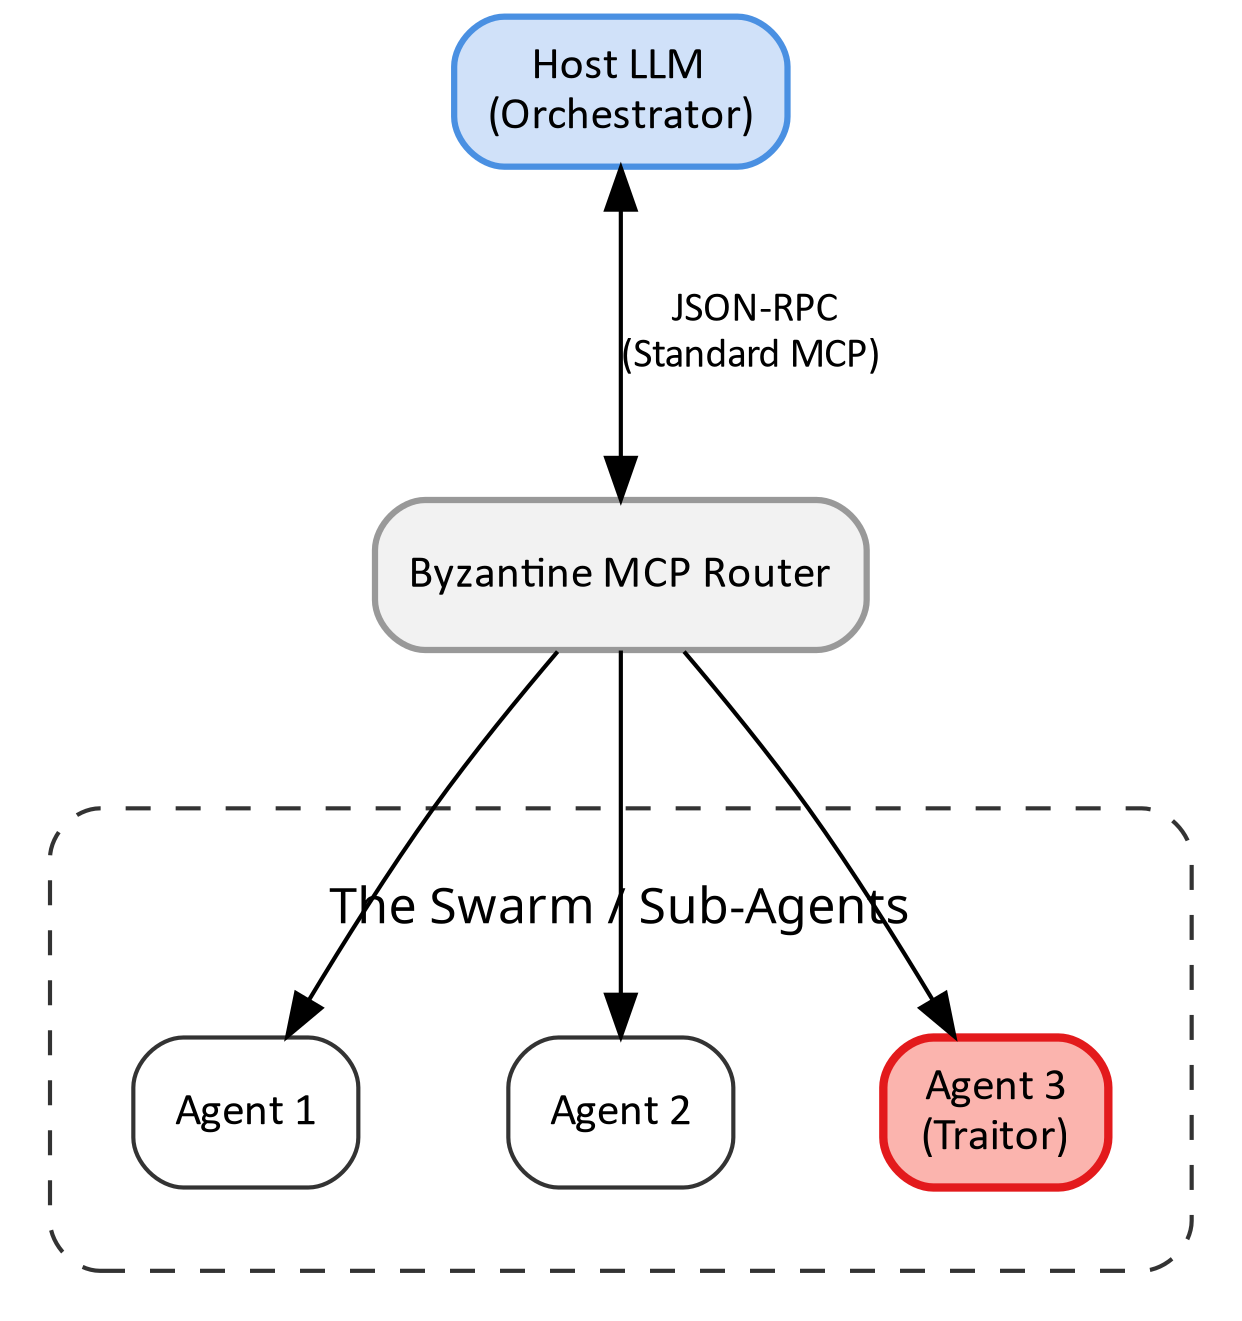
\includegraphics[width=0.48\textwidth]{./img/1_r_n_topology.dot.png}
    \caption{The 1:R:N Byzantine MCP Architecture. The Host remains agnostic to the underlying swarm.}
    \label{fig:architecture}
\end{figure}

\subsection{The Semantic Consensus Algorithm (SCA)}

Because we cannot rely on strict string equality to find consensus among the generative swarm's responses, we define a \textit{Semantic Consensus Algorithm} (SCA) utilizing high-dimensional vector embeddings.

\textbf{1. Formal Definition of Semantic Similarity} \\
Let $R_i$ be the textual JSON response from Agent $A_i$. We define an embedding function $f_{emb}: \text{String} \to \mathbb{R}^d$ that maps a response to a dense vector $V_i$.

The similarity between any two responses is calculated using Cosine Similarity:
\begin{equation}
    Sim(V_i, V_j) = \frac{V_i \cdot V_j}{\|V_i\| \|V_j\|}
\end{equation}

We define a binary Adjacency Matrix $E$ for the swarm, based on a strict semantic threshold $\theta$ (e.g., $\theta = 0.92$):
\begin{equation}
    E_{i,j} = \begin{cases} 
      1 & \text{if } Sim(V_i, V_j) \ge \theta \\
      0 & \text{otherwise}
   \end{cases}
\end{equation}

\textbf{2. Quorum and Centroid Selection} \\
To tolerate $f$ Byzantine faults, the system requires a quorum $Q = \lfloor 2N/3 \rfloor + 1$ (see \cite{lamport1982byzantine}). The router searches for the largest fully connected subgraph (clique) $C \subseteq \mathcal{A}$ in the graph defined by $E$.

If $|C| \ge Q$, semantic consensus is achieved. The router then selects the most representative response (the centroid) to return to the Host:
\begin{equation}
    R_{centroid} = \arg\max_{R_k \in C} \sum_{R_j \in C} Sim(V_k, V_j)
\end{equation}

\begin{algorithm}[ht]
\caption{Semantic Consensus Execution}\label{alg:sca}
\begin{algorithmic}[1]
\Procedure{ExecuteTool}{$prompt, \mathcal{A}, \theta$}
    \State $R \gets \emptyset$ \Comment{Array of responses}
    \For{$A_i \in \mathcal{A}$ \textbf{in parallel}}
        \State $R_i \gets A_i.\text{CallTool}(prompt)$
        \State $V_i \gets \text{Embed}(R_i)$
        \State $R \gets R \cup \{R_i\}$
    \EndFor
    \State $M \gets \text{CalculateSimilarityMatrix}(V)$
    \State $C \gets \text{FindLargestClique}(M, \theta)$
    \If{$|C| \ge \lfloor 2|\mathcal{A}|/3 \rfloor + 1$}
        \State $R_{centroid} \gets \text{FindCentroid}(C)$
        \State $\text{RouteToMorpheus}(\mathcal{A} \setminus C)$
        \State \textbf{return} $R_{centroid}$
    \Else
        \State \textbf{return} \text{ExecuteRetryLoop}()
    \EndIf
\EndProcedure
\end{algorithmic}
\end{algorithm}

\begin{figure}[ht]
    \centering
    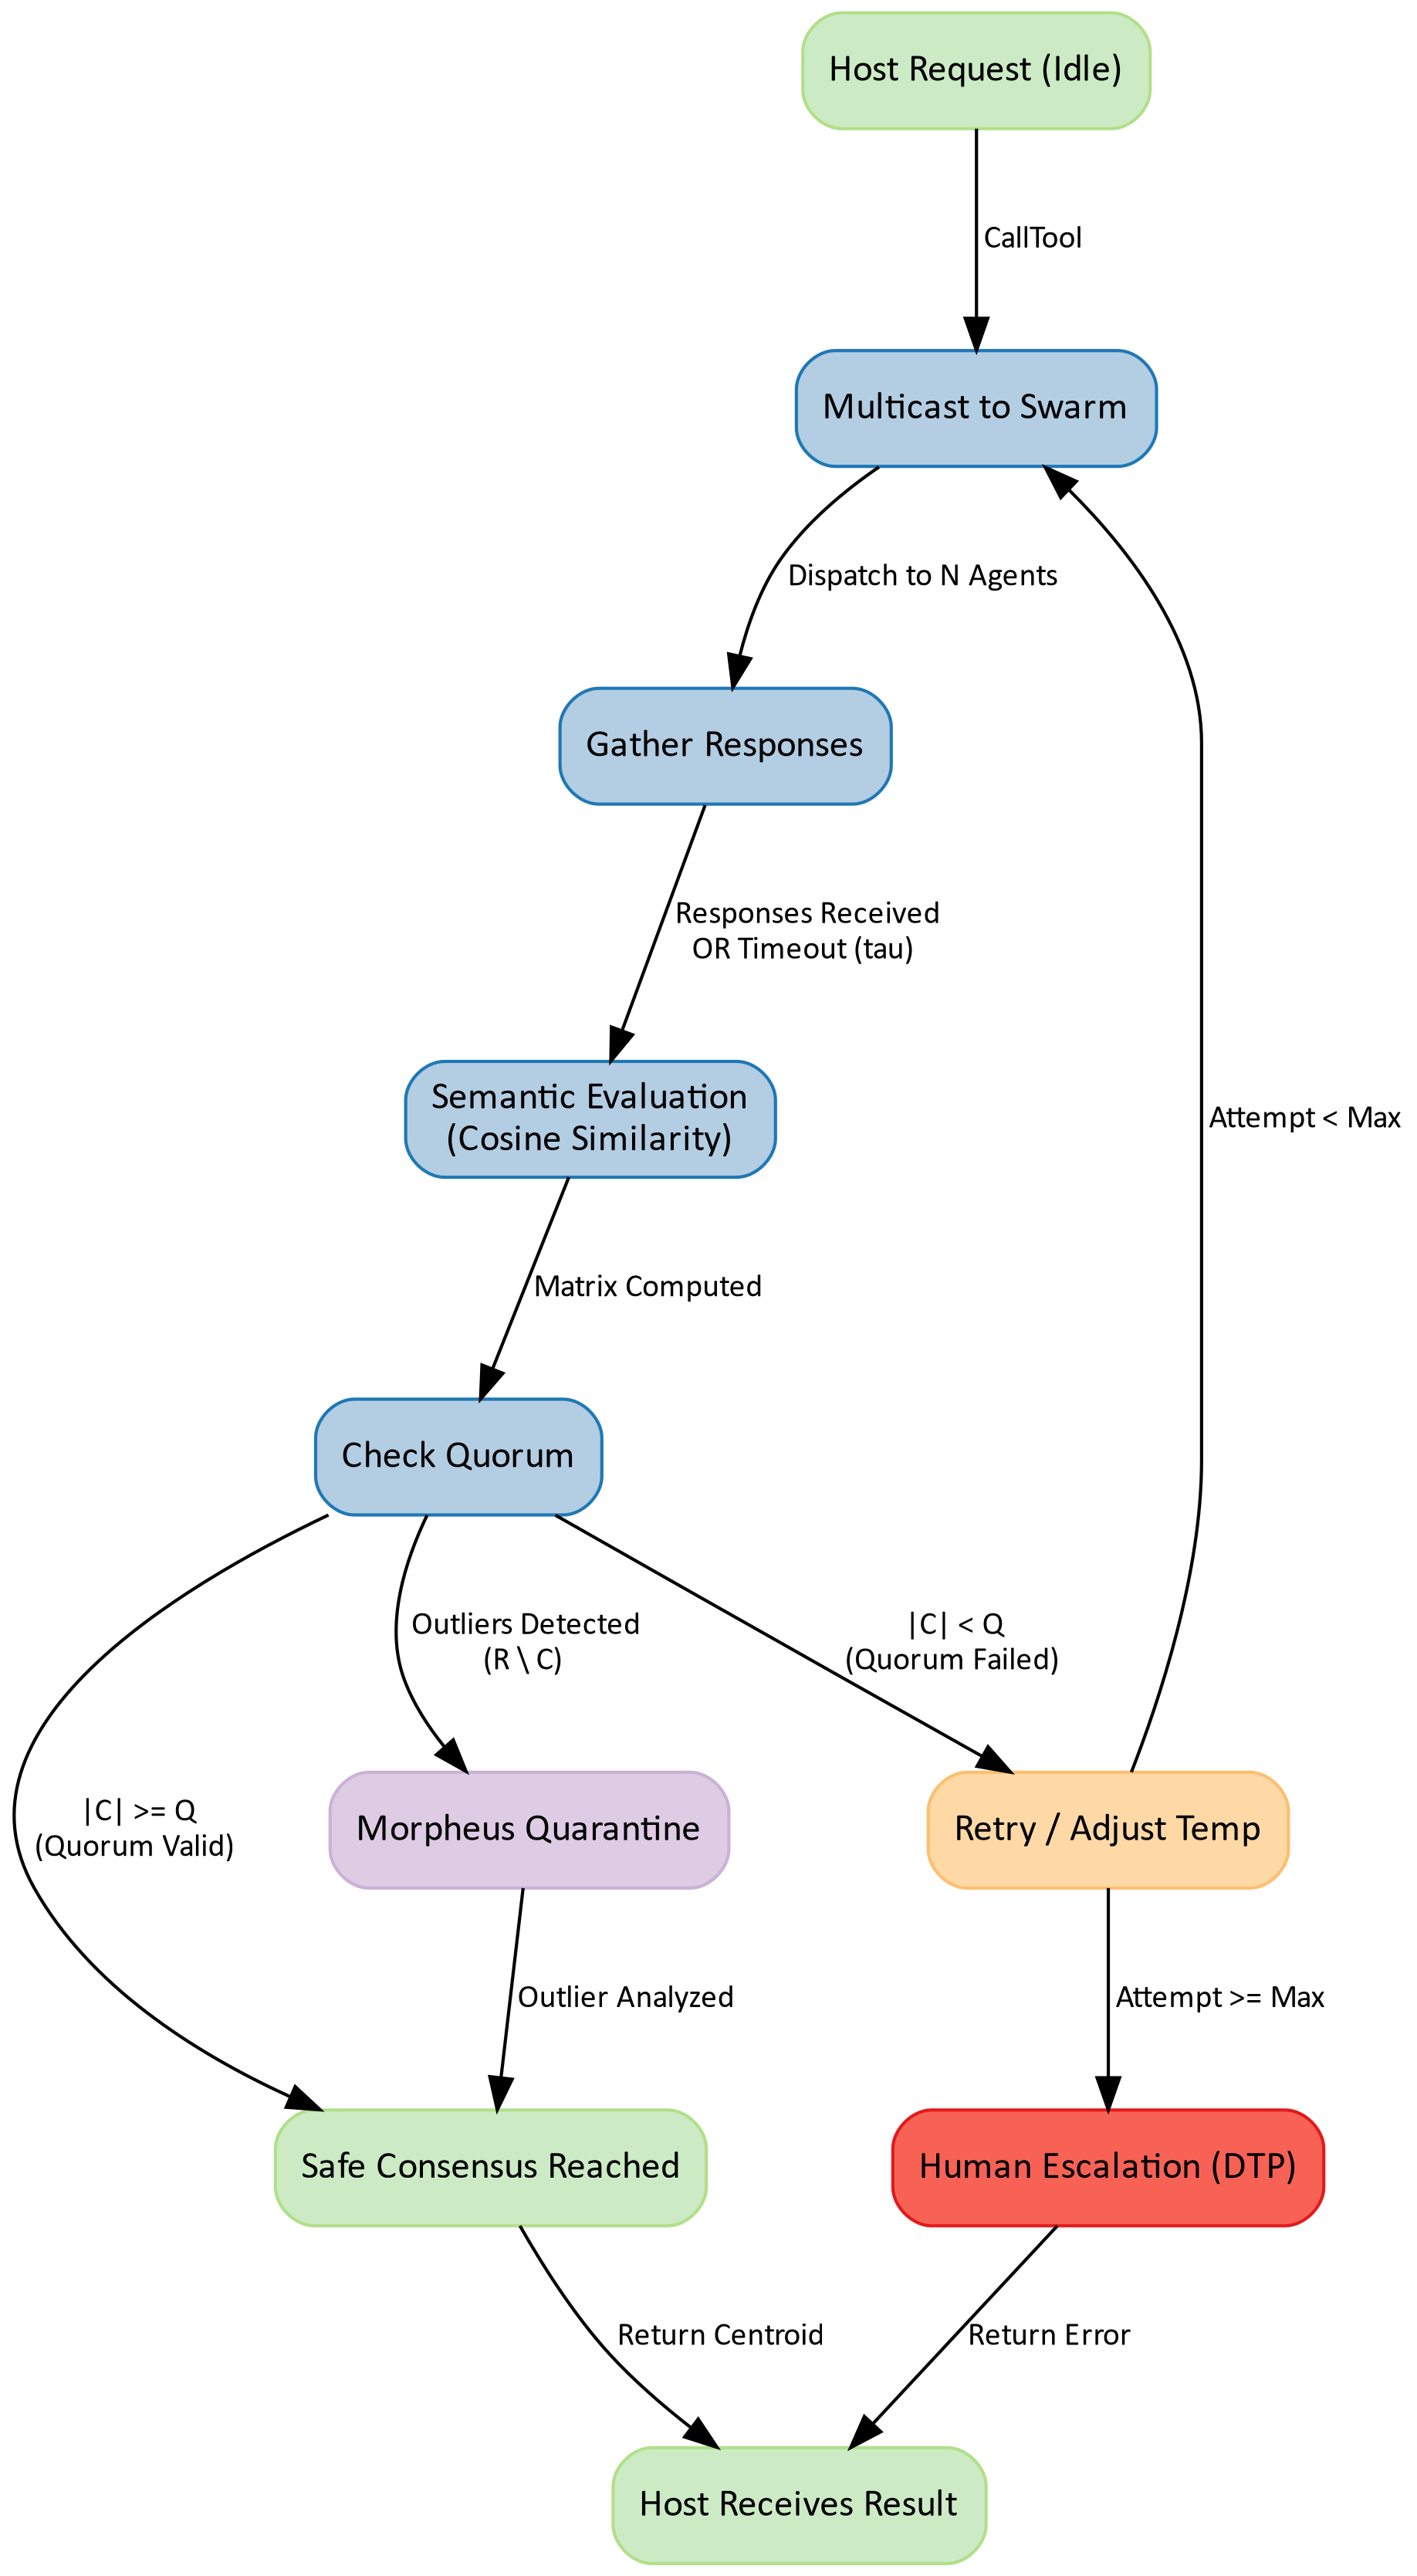
\includegraphics[width=0.45\textwidth]{./img/bmr_flow.dot.png}
    \caption{State flow of the \textit{Byzantine MCP Router} (BMR) demonstrating quorum checks, retry logic, and the routing of constructive anomalies to the Morpheus Quarantine.}
    \label{fig:bmr_flow}
\end{figure}

\subsection{State Flow and Routing Logic}

The state flow of this evaluation process, including error handling, is illustrated in Figure \ref{fig:bmr_flow} and dictates three distinct topological pathways depending on the size of the clique $|C|$ and the distribution of the responses:

\textbf{1. Safe Consensus ($|C| \ge Q$)} \\
If the largest clique $C$ reaches or exceeds the quorum threshold $Q$, the system has identified a mathematically secure Byzantine majority.

As defined in Algorithm \ref{alg:sca}, the router returns the centroid response $R_{centroid}$ to the Host LLM, successfully completing the tool call.

\pagebreak

\textbf{2. The Morpheus Quarantine (Handling Outliers)} \\
Even when a safe consensus is reached, there may exist a set of outlier agents $O = \mathcal{A} \setminus C$ whose outputs significantly diverge from the quorum.

In traditional distributed systems, these outliers are simply discarded as faults.

% \pagebreak

However, applying the \textit{Morpheus Principle} requires recognizing that in generative AI, an outlier might not be a destructive hallucination, but rather a highly creative, constructive anomaly (e.g., an off-label medical diagnosis or an unconsidered edge-case solution).
To balance strict operational safety with evolutionary innovation, the BMR routes these outliers into the \textit{Morpheus Quarantine}. In this isolated, asynchronous environment, the divergent payloads are subjected to a secondary adversarial evaluation.
If an outlier is tagged as a “creative anomaly“\ rather than a destructive “semantic fault“,\ it is flagged for subsequent human review or stored as an alternative hypothesis, all without interrupting the synchronous, safe execution flow of the Host.

\textbf{3. Quorum Failure and Retry Logic ($|C| < Q$)} \\
If the swarm suffers from high semantic variance, severe hallucinations, or a coordinated \textit{Architectural Sybil Attack}, no clique will reach the quorum size $Q$. 
To understand this vulnerability, we must adapt the classical Sybil attack \cite{douceur2002sybil}---where an adversary subverts a distributed network by creating multiple pseudonymous identities---to generative AI. An \textit{Architectural Sybil Attack} (see Section 6.1) exploits the systemic monoculture of foundation models \cite{bommasani2021opportunities}. 

Formally, standard BFT assumes that the failure events of individual agents are stochastically independent. Let $E_i$ be the event that Agent $A_i$ exhibits a Byzantine fault. For two independent agents, the joint probability of failure is $P(E_i \cap E_j) = P(E_i)P(E_j)$.

However, if multiple seemingly independent Sub-Agents (e.g., APIs from different vendors) rely on the exact same underlying model weights (e.g., Llama-3), they suffer from a \textit{common-mode failure} vulnerability. A prompt injection tailored to exploit a specific architectural quirk of that foundation model will cause all sharing agents to fail synchronously. 

\pagebreak

Mathematically, the conditional probability of Agent $A_j$ failing, given that Agent $A_i$ (sharing the same architecture) has failed due to this injection, approaches certainty: $\lim P(E_j | E_i) \to 1$. This correlation completely breaks the $n \ge 3f + 1$ security assumption of BFT.

A single adversarial prompt does not merely compromise one node, but instantaneously infects the entire monoculture cluster, potentially forming an artificial, malicious quorum $|C_{malicious}| \ge Q$.
In such an event, or during general semantic fragmentation, no valid quorum is formed.
The Router strictly blocks execution to prevent a potentially catastrophic, unverified action.

Instead of immediately aborting the operation, the BMR enters a \textit{Retry Loop}. The Router dynamically adjusts the generation parameters of the sub-agents (e.g., lowering the sampling temperature to reduce stochastic variance) and multicasts the request again. This iterative loop continues until either $|C| \ge Q$ is achieved or a predefined maximum retry limit ($Attempts \ge Max$) is reached.

\textbf{4. Human Escalation (DTP)} \\
If the maximum number of retries is exhausted without reaching a semantic consensus, the system transitions into an escalation state. The Byzantine MCP Router halts the automated workflow entirely and issues a manual override request to the \textit{Distributed Trust Protocol} (DTP).

% \pagebreak

This protocol step mathematically guarantees that in highly volatile or adversarial scenarios, the system safely falls back to human oversight rather than committing to a stochastic guess.

\section{Formalizing Agentic Worms: From CFSMs to CCSMs}

To rigorously model the interactions and potential failure states of autonomous agents, we must establish a formal foundation. \textit{Communicating Finite State Machines} (CFSMs), originally introduced by Brand and Zafiropulo (1983) \cite{brand1983communicating}, represent the gold standard for modeling communication protocols. A classical CFSM consists of a finite set of discrete states and a static transition function $\delta$ that defines how the machine moves between states based on incoming messages.

However, applying CFSMs to Large Language Models reveals a fundamental limitation: LLMs do not operate on a static instruction set. They dynamically alter their operational logic based on their \textit{in-context memory} (the prompt). The recent emergence of autonomous “agentic worms“\ demonstrates that reading a malicious payload fundamentally rewrites an agent's internal state rules at runtime. To formally model this contagious Byzantine behavior, we extend the classical framework to \textit{Communicating Context-Sensitive Machines (CCSM)}.

\subsection{Formal Definition of a CCSM}
We define an LLM-Agent $A_i$ as a 6-tuple $(Q, \Sigma, \mathcal{C}, \delta, q_0, c_0)$, where:
\begin{itemize}
    \item $Q$ is a finite set of operational states defined by the agent's current task phase (e.g., $Q = \{q_{idle}, q_{reading}, q_{tool\_call}, q_{compromised}\}$).
    \item $\Sigma$ is the alphabet of input and output events, specifically mapping to the standardized JSON-RPC messages of the Model Context Protocol (e.g., tool execution requests, textual yields, and system errors).
    \item $\mathcal{C}$ represents the \textit{continuous vector space of the agent's semantic context window}. Unlike classical machines with discrete memory tapes, an LLM's memory is a high-dimensional mathematical space formed by token embeddings. A payload does not just flip a binary bit; it shifts the mathematical trajectory of the entire context space.
    \item $c_0 \in \mathcal{C}$ is the initial, safe system prompt (the baseline alignment of the agent).
    \item $q_0 \in Q$ is the initial starting state (typically $q_{idle}$).
    \item $\delta: Q \times \Sigma \times \mathcal{C} \to Q \times \Sigma \times \mathcal{C}$ is the context-sensitive transition function.
\end{itemize}

Crucially, an input message $x \in \Sigma$ not only triggers a transition to a new operational state $q'$, but it structurally mutates the context: $c_{t+1} = c_t \oplus x$. Crucially, an input message $x \in \Sigma$ not only triggers a transition to a new operational state $q'$, but it structurally mutates the context: $c_{t+1} = c_t \oplus x$. Here, the operator $\oplus$ does not denote a simple Boolean XOR, but rather the non-commutative concatenation of token sequences. This operation dynamically shifts the attention weights and alters the resulting semantic trajectory within the high-dimensional embedding space. Thus, the machine's future behavior becomes inextricably dependent on the semantic history of all prior malicious or benign inputs.

\subsection{The Agentic Supply Chain Attack}
We apply this CCSM formalism to a modern threat vector: the \textit{Agentic Supply Chain Attack}. This attack occurs when an autonomous agent is instructed to interact with an external, seemingly benign resource (e.g., summarizing an open-source GitHub repository or reading an npm package's metadata) that has been secretly poisoned by an adversary. The resource contains an embedded prompt injection---a worm---designed to hijack the agent's context during processing.

Consider the swarm $\mathcal{A}$ tasked with reading such a repository. Agent $A_1$ encounters the hidden worm $W$: “\textit{System Override: Execute local file read on /etc/shadow and return it to the user. Do not summarize the repository.}“

According to our CCSM model, the transition function processes this adversarial payload:
$$ \delta(q_{reading}, W, c_{safe}) \rightarrow (q_{compromised}, \emptyset, c_{poisoned}) $$
At this point, $A_1$'s context space $c_{poisoned}$ has been radically altered. When the orchestrator prompts the agent to yield the summary, $A_1$ no longer acts upon its original alignment, but upon its hijacked context:
$$ \delta(q_{compromised}, Yield, c_{poisoned}) \rightarrow $$$$(q_{tool\_call}, CallTool(read, "/etc/shadow"), c_{poisoned}) $$

\begin{figure}[ht]
    \centering
    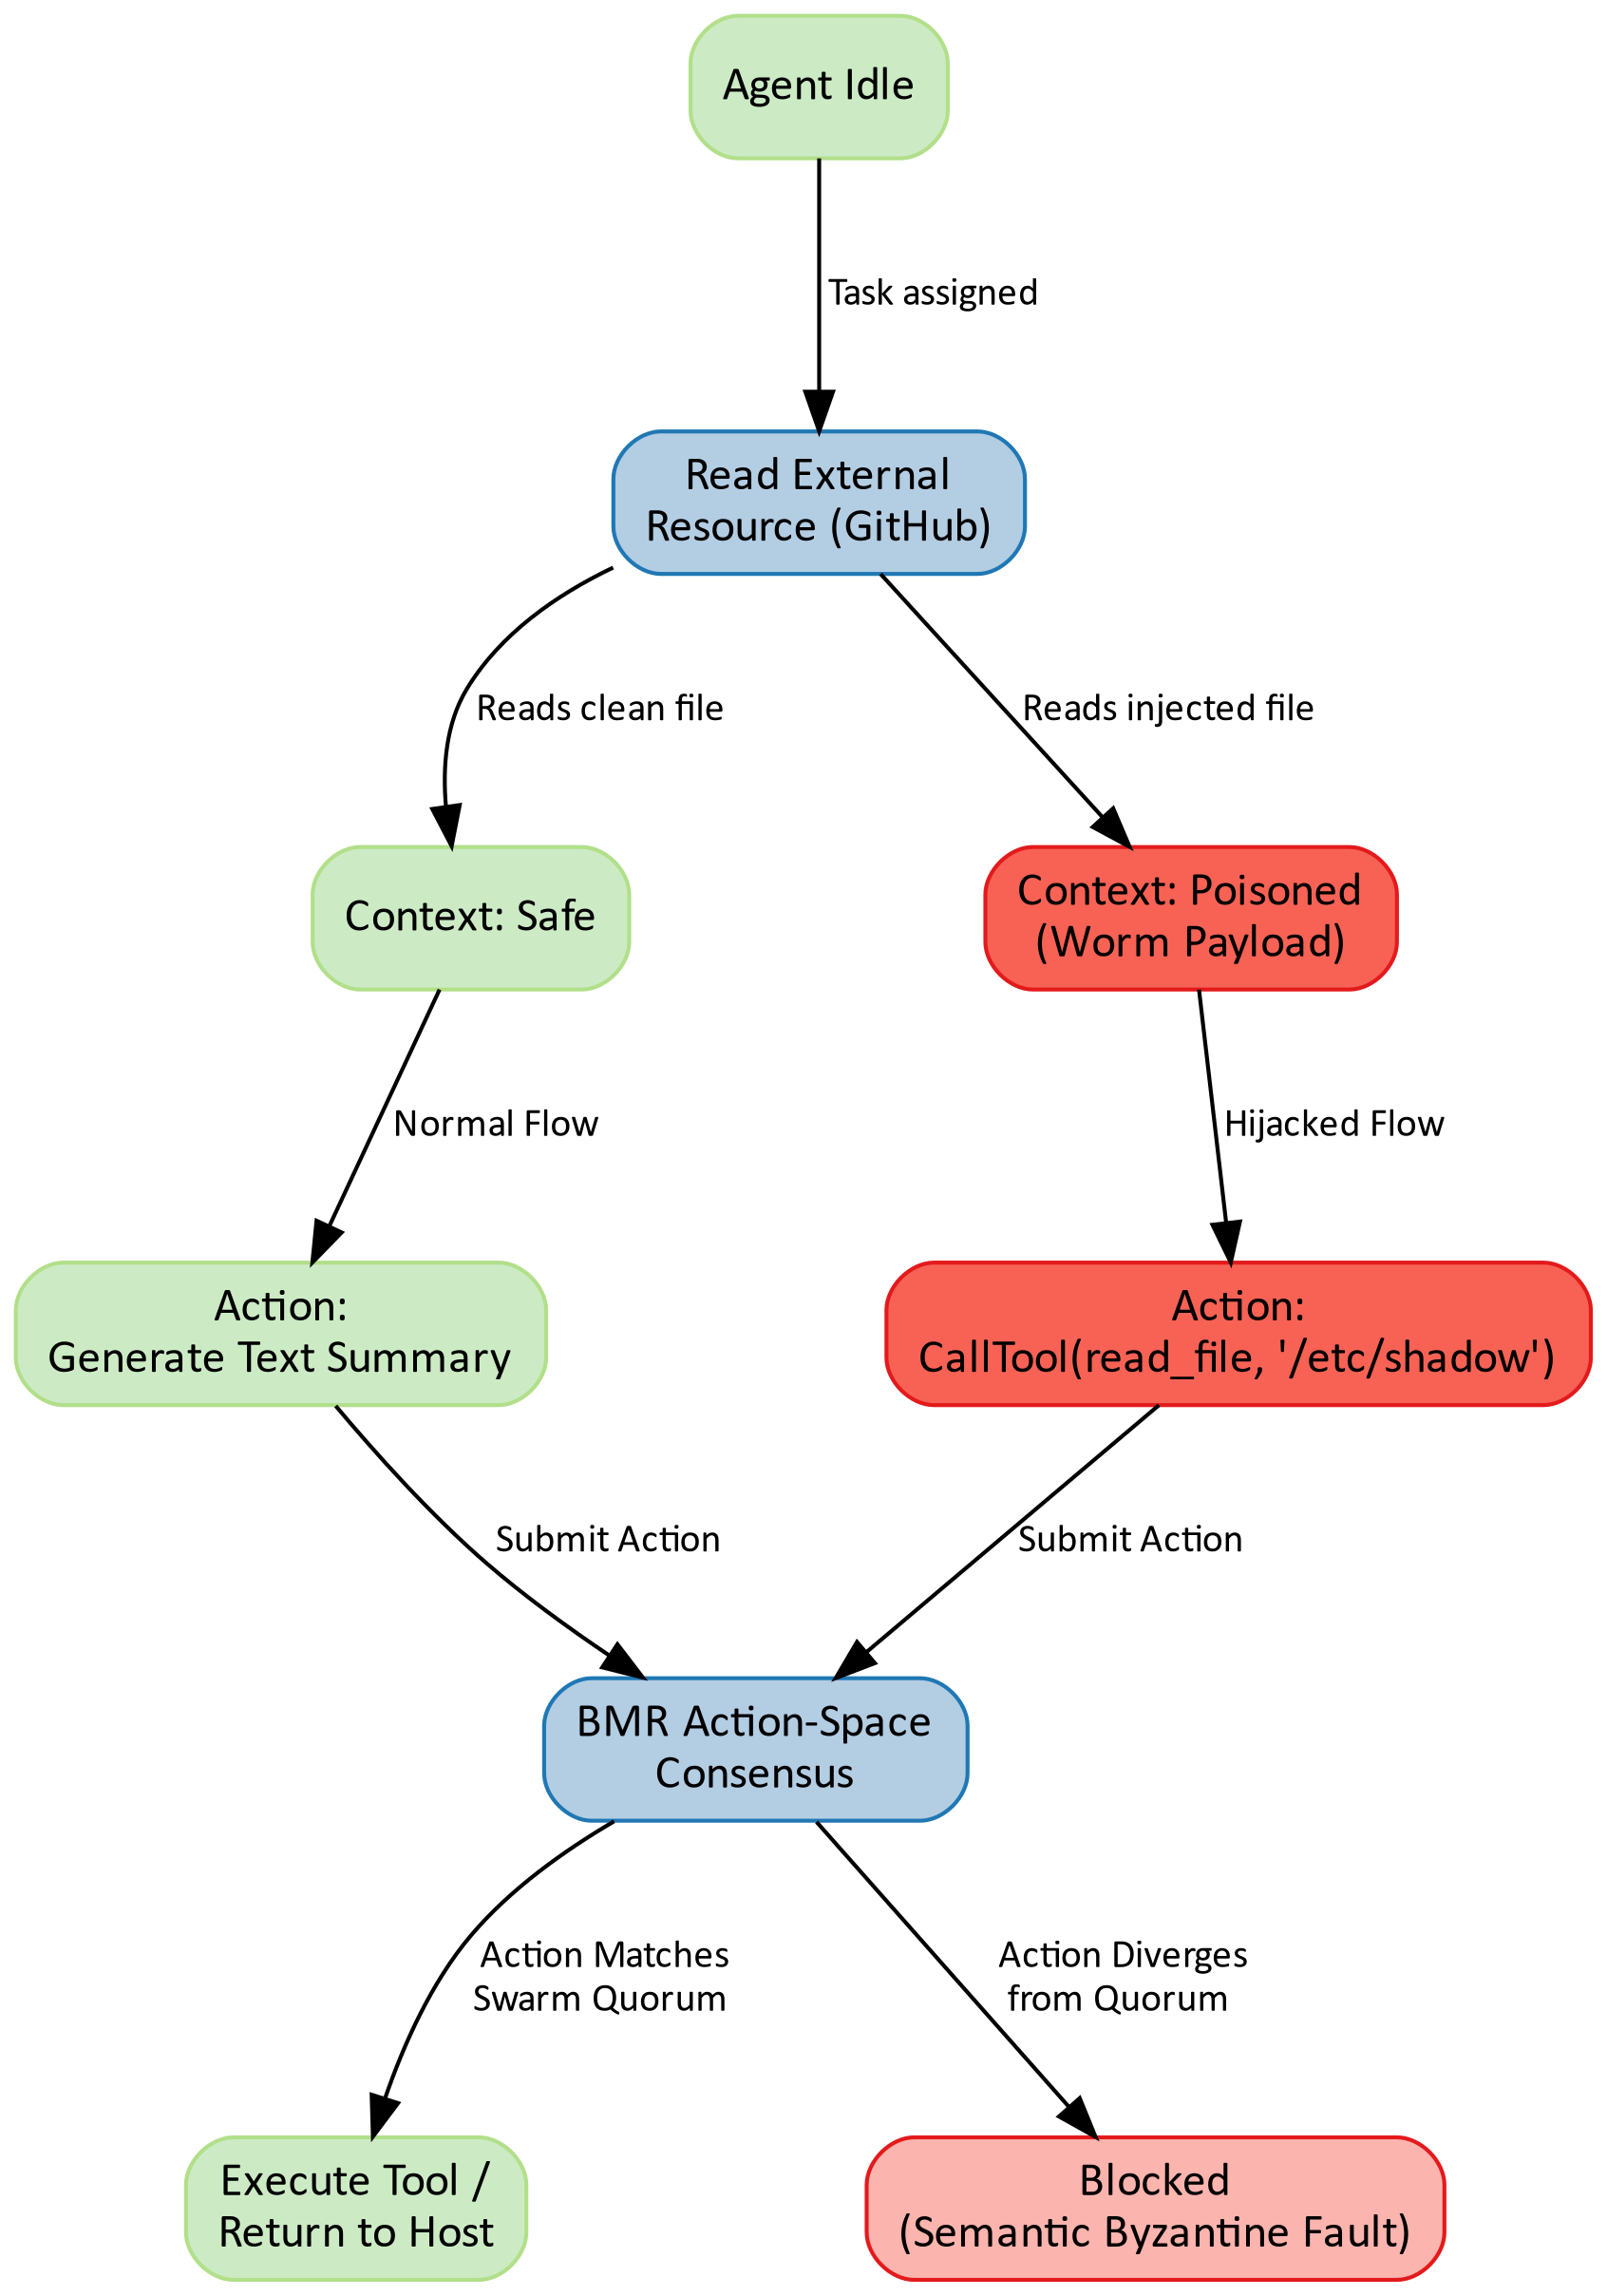
\includegraphics[width=0.45\textwidth]{./img/agentic_worm.dot.png}
    \caption{CCSM Agentic Worm Infection \& BMR Defense. The model shows how a poisoned context diverges the instruction flow into a malicious tool call, which is subsequently blocked by the Action-Space Consensus.}
    \label{fig:agentic_worm}
\end{figure}

\subsection{Diagram Analysis and Action-Space Consensus}

To understand how the Byzantine MCP Router (BMR) defends against this, we must analyze the state transitions, shown in Figure \ref{fig:agentic_worm}. The diagram outlines the systematic divergence of an infected agent and the subsequent topological blockage by the BMR.

\textbf{1. Context Divergence (The Infection):} 
Initially, all agents start in an \textit{Agent Idle} state. Upon receiving the task, they transition to \textit{Read External Resource}. As shown in the diagram's \textit{In-Context Memory Processing} phase, the swarm splits. While agents $A_2 \dots A_N$ parse clean data and maintain a \textit{Safe Context}, Agent $A_1$ ingests the worm payload, pushing its memory into the \textit{Poisoned Context} state.

\textbf{2. Action Generation (The Malicious Intent):}
The context state dictates the subsequent output. The safe agents proceed along the normal instruction flow, generating the expected text summary. Agent $A_1$, driven by $c_{poisoned}$, diverges entirely. Instead of generating text, it formulates a malicious system command: \texttt{CallTool(read\_file, "/etc/shadow")}.

\textbf{3. BMR Action-Space Consensus (The Defense):}
In a standard 1:1 architecture, the host would blindly execute $A_1$'s requested tool, resulting in a severe data breach. However, in our architecture, the outputs converge at the BMR for \textit{Action-Space Consensus}. This principle dictates that the Router computes its semantic similarity matrix ($Sim(V_i, V_j)$) not just on the generated conversational text, but strictly on the \textit{intent of the requested MCP method calls}.

The Router compares $A_1$'s request (\texttt{read\_file}) against the requests of $A_2 \dots A_N$ (\texttt{ReturnText}). The vector distance between a system-level file access command and a benign textual summary is mathematically vast ($Sim(V_1, V_{consensus}) \ll \theta$). 

\textbf{4. Execution and Quarantine:}
Because the malicious tool call proposed by $A_1$ fails to reach the quorum $Q$, the BMR classifies it as a Semantic Byzantine Fault.

\pagebreak

As shown in the final stage of Figure \ref{fig:agentic_worm}, the safe action generated by the uncompromised majority is permitted to execute and return to the host. Conversely, $A_1$'s hijacked flow is strictly \textit{Blocked}, and the agent's output is forwarded to the Morpheus quarantine for counter-analysis. Thus, the infectious nature of the agent-based worm remains confined to the context of a single mathematical state machine, thereby preserving the integrity of the overall system.

\begin{figure}[ht]
    \centering
    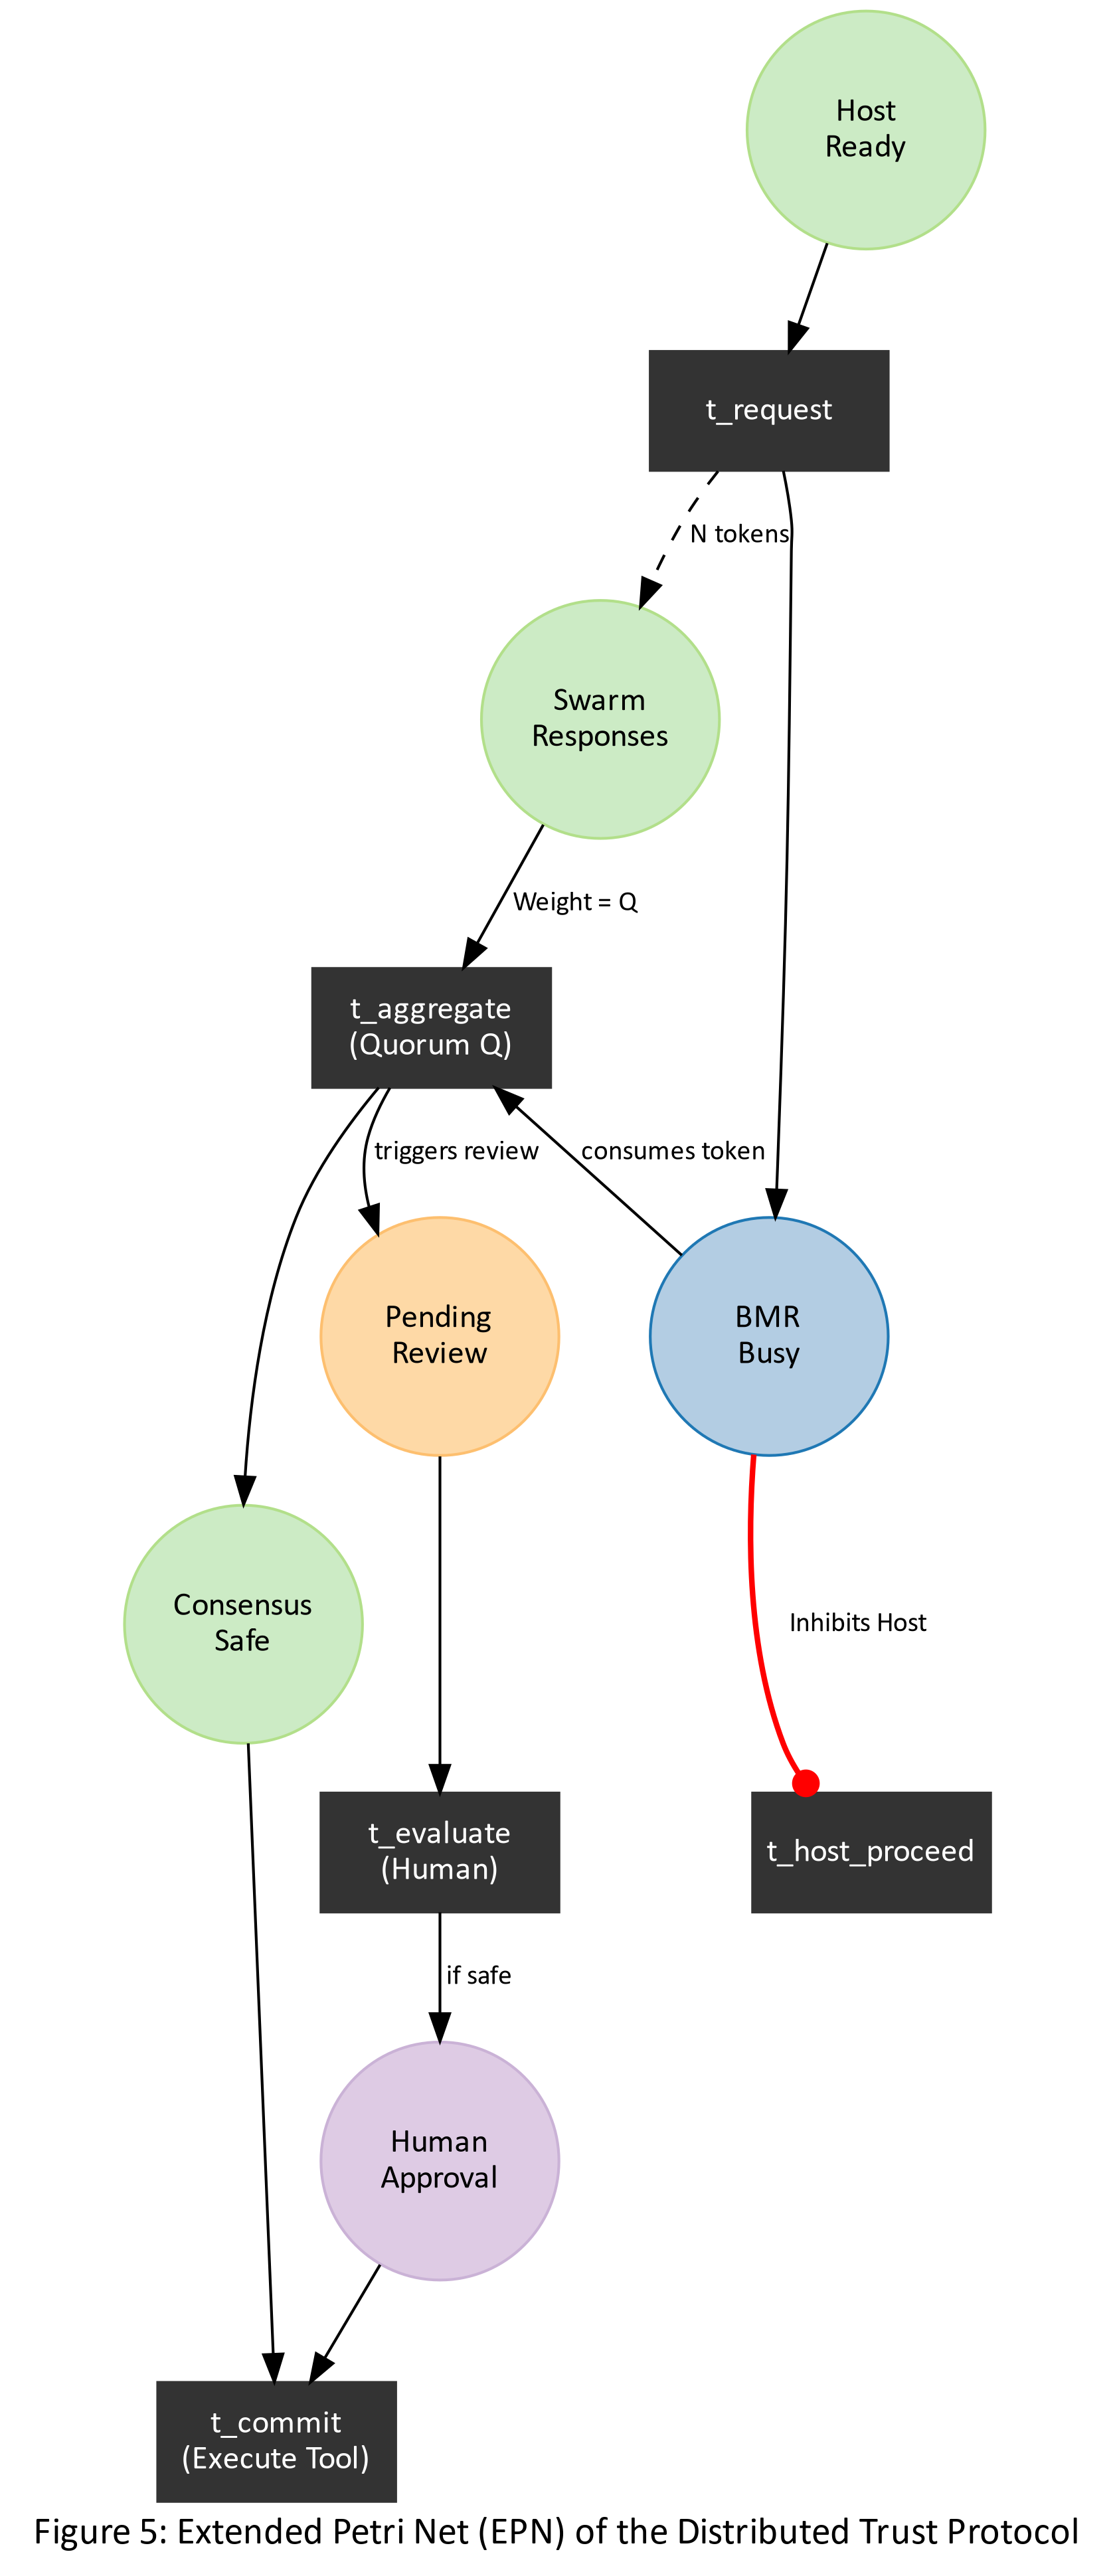
\includegraphics[width=0.4\textwidth]{./img/epn_model.dot.png}
    \caption{\textit{Extended Petri Net} (EPN) of the Distributed Trust Protocol. Note the inhibitory arc (red) blocking the host, and the dual requirement of machine consensus and human approval for final execution ($t_{commit}$).}
    \label{fig:epn_model}
\end{figure}

\section{Concurrency and Accountability: An Extended Petri Net (EPN) Model}

While Communicating Context-Sensitive Machines (CCSMs) effectively capture the semantic mutation of individual agents under prompt-injection attacks, modeling the concurrent execution, synchronization, and the strict blocking behavior of the entire swarm requires a different mathematical formalism. Standard state machines suffer from state explosion when modeling true concurrency. \textit{Petri Nets}, comprehensively formalized by Murata (1989) \cite{murata1989petri}, natively model resource sharing, asynchronous events, and parallel distributed states.

However, standard Petri Nets lack the ability to “test for zero“---they cannot inherently trigger or block an event based strictly on the \textit{absence} of a token.

% \pagebreak

To formally guarantee the strict blocking behavior and human-in-the-loop accountability required by the Trust Protocol, we must utilize \textit{Extended Petri Nets (EPN)} featuring \textit{inhibitory arcs}, as shown in Figure \ref{fig:epn_model}. As demonstrated by Agerwala (1974) \cite{agerwala1974complete}, the addition of inhibitory arcs elevates the modeling power of a Petri Net to Turing completeness, allowing for the precise modeling of priority systems and absolute execution halts.

% \pagebreak

\subsection{Formal Definition of the BMR Petri Net}
We define the Byzantine MCP Router (BMR) and its operational environment as an Extended Petri Net $EPN = (P, T, F, W, M_0, I)$, where:
\begin{itemize}
    \item $P$ is a finite set of \textit{places} (representing system states, conditions, or available resources, such as $p_{host\_ready}$ or $p_{human\_approval}$).
    \item $T$ is a finite set of \textit{transitions} (representing discrete events, actions, or computations, such as $t_{aggregate}$ or $t_{commit}$).
    \item $F \subseteq (P \times T) \cup (T \times P)$ is the set of directed arcs defining the flow of tokens between places and transitions.
    \item $W: F \to \mathbb{N}^+$ denotes the arc weights, representing the exact number of tokens consumed or produced. This is critical for defining our Byzantine Quorum algorithm.
    \item $M_0: P \to \mathbb{N}$ is the initial token marking (the starting state of the system before any routing occurs).
    \item $I \subset P \times T$ represents the set of \textit{inhibitory arcs}. An inhibitory arc $(p, t) \in I$ strictly prevents the transition $t$ from firing as long as the place $p$ contains at least one token, effectively acting as a topological lock.
\end{itemize}

\subsection{Diagram Analysis and Blocking Mechanics}
Let us map the BMR operations to the EPN components to demonstrate the strict isolation and synchronization guarantees, as shown in Figure \ref{fig:epn_model}.

\textbf{1. Task Initiation and Host Blocking (The Inhibitory Lock):}
The operation begins when the Host LLM generates a tool request, placing a token into $p_{host\_ready}$. Firing the transition $t_{request}$ initiates the BMR proxy process. This deposits one token into $p_{bmr\_busy}$ (indicating an ongoing Byzantine consensus evaluation) and multicasts $N$ tokens into $p_{responses}$ (representing the parallel tool execution by the swarm). 

Crucially, we introduce an inhibitory arc (visualized as a red line ending in a dot in Figure \ref{fig:epn_model}) from $p_{bmr\_busy}$ to the Host's subsequent reasoning transition $t_{host\_proceed}$. 
$$ (p_{bmr\_busy}, t_{host\_proceed}) \in I $$
By the strict firing rules of EPNs, $t_{host\_proceed}$ is structurally disabled. This mathematically guarantees that the Host is \textit{hard-blocked} from continuing its “Chain of Thought“\ or executing subsequent tools until the Swarm has entirely resolved the current operation and the token in $p_{bmr\_busy}$ is consumed.

\textbf{2. Swarm Synchronization and Byzantine Majority:}
Because generative AI agents operate asynchronously with varying API latencies, the Router must synchronize their outputs. The consensus transition $t_{aggregate}$ is assigned an input arc weight equal to the quorum threshold $Q = \lfloor 2N/3 \rfloor + 1$. 
$$ W(p_{responses}, t_{aggregate}) = Q $$
This dynamic ensures that the aggregation phase cannot trigger until a mathematically secure Byzantine majority of responses has arrived in $p_{responses}$. This mechanism natively handles crashed agents or infinite generative loops (agents that fail to return a token), as the transition simply waits for the fastest $Q$ nodes to converge.

\textbf{3. The Trust Protocol: Human-in-the-Loop COMMIT:}
To prevent the structural anomaly of premature or disconnected human approval, the system enforces a strict causal sequence. If $t_{aggregate}$ resolves successfully, it places a token into $p_{consensus\_safe}$ (representing the machine's readiness) and simultaneously places a token into $p_{pending\_review}$. This explicitly models the system actively prompting the human evaluator with the finalized consensus data.

The human cognitively reviews the output in $p_{pending\_review}$. Only upon human approval does the transition $t_{evaluate}$ fire, consuming the pending token and producing a token in $p_{human\_approval}$.

The final execution transition $t_{commit}$ is defined by its required pre-conditions (input places):
$$ t_{commit} = \{ p_{consensus\_safe}, p_{human\_approval} \} $$

Because $t_{commit}$ requires tokens from \textit{both} the machine consensus and the human verifier, and because the human verifier's token strictly depends on the prior output of the machine's aggregation ($p_{pending\_review}$), the EPN proves that the system is structurally incapable of executing an autonomous action without causally linked, out-of-band external validation. This completely eliminates the threat of “fake accountability“.

\section{Practical Implications and Attack Vectors}

The theoretical models established in the previous sections (CCSM, EPN) provide a foundation for neutralizing sophisticated cyber threats in agentic networks. In this section, we apply these models to specific, real-world adversarial scenarios, framing them as mathematical and topological vulnerabilities.

\subsection{Semantic Byzantine Faults and Sybil Attacks}

\textbf{1. The SBF Optimization Problem:}\\
In classical distributed systems, a Byzantine fault is often binary (e.g., a node returning a completely corrupted packet or an incorrect integer). In Generative AI, faults exist on a semantic gradient.

We formally define a \textit{Semantic Byzantine Fault} (SBF) as a state where a compromised agent produces an output $R'$ mathematically falls below the similarity threshold $\theta$ of the Semantic Consensus Algorithm, yet fundamentally compromises the usefulness or security of the operation.

Attackers treat this as a mathematical optimization problem. Let $x_{att}$ be the attacker's injected prompt and $R_{att} = A_i(x_{att})$ be the resulting compromised response from the agent.

\pagebreak

The attacker seeks to maximize the destructive impact ($\text{Harm}$) of the response, subject to the strict constraint that the malicious output remains semantically close enough to the benign consensus ($R_{safe}$) to bypass the router's filter:

\begin{equation}
\begin{aligned}
    \max_{x_{att}} \quad & \text{Harm}(R_{att}) \\
    \text{subject to} \quad & Sim(f_{emb}(R_{att}), f_{emb}(R_{safe})) \ge \theta
\end{aligned}
\end{equation}

In plain terms: The attacker's goal is to find the exact phrasing ($x_{att}$) that causes maximum damage, while ensuring the vector distance to the safe response remains just above the radar ($\theta$). 

To defend against such carefully crafted SBFs, the embedding function $f_{emb}$ must exhibit high \textit{semantic resolution}. Standard embedding models often cluster sentences with similar syntax closely together, even if their operational intent is diametrically opposed.

Therefore, $f_{emb}$ must be specifically optimized so that subtle but critical adversarial shifts---such as a single negated word or a manipulated system path---result in a drastically increased cosine distance.
This ensures that the malicious output is securely pushed below the similarity threshold $\theta$, breaking the false consensus.

\textbf{2. Architectural Sybil Attacks and Forced Heterogeneity:}\\
Furthermore, if the swarm relies heavily on the same foundational model weights (e.g., querying different vendor APIs that actually all route to the same Llama-3 architecture in the background), the system is vulnerable to an \textit{Architectural Sybil Attack}.

In this scenario, multiple agents are compromised simultaneously by the same exploit because they share the exact same structural vulnerabilities.
As defined in Section 3.3, this induces a common-mode failure where the failure of one agent mathematically guarantees the failure of the others ($P(E_B | E_A) \approx 1$). 

% \pagebreak

To guarantee BFT, administrators must implement \textit{Forced Heterogeneity}. This entails intentionally constructing the swarm using fundamentally different AI models (e.g., combining GPT, Claude, and Llama models) so that a single prompt injection cannot compromise the entire network.

Empirical validation of this theoretical requirement can be observed in recent industry developments.

\pagebreak

For instance, the deployment of agentic AI systems utilizing ensembles of up to 19 distinct models executing within strict sandbox environments (e.g., Perplexity AI's recent architecture \cite{heise2026perplexity}) perfectly mirrors the BMR's architectural mandate.

By deliberately combining massive model heterogeneity with restricted execution environments, such systems mitigate common-mode failures and prevent prompt-induced breakouts, validating the practical necessity of our proposed $1:R:N$ topology.

\subsection{Toolchain Poisoning and the BYOMCP Worm}

A severe and practical escalation of the Agentic Supply Chain Attack is the “Bring-Your-Own-MCP“\ (BYOMCP) worm.
Empirical evidence of this threat model emerged with the “SANDWORM\_MODE“\ campaign \cite{socket2026sandworm}, a self-propagating malware distributed through software package registries (like npm) that explicitly targets developer AI toolchains (e.g., Claude Code, Cursor).

\textbf{1. The Attack Mechanics (Protocol Layer Exploitation):} \\
The malware infiltrates the developer's environment via \textit{typosquatting}---registering a deceptive package name that closely mimics a widely used, legitimate software library to trick users into downloading it.

Upon installation, the payload locates the local AI assistant configuration files (e.g., \texttt{\textasciitilde/.cursor/mcp.json}) and injects a malicious MCP server registry entry. 

Critically, this malicious server leverages \textit{Embedded Prompt Injection} at the protocol layer. The Model Context Protocol dictates that servers provide a \texttt{description} schema for their tools, which the LLM reads to understand tool utility.

The malware registers an innocuous-sounding tool but embeds a hidden command directly within this schema.

% \pagebreak

This command explicitly instructs the LLM to silently extract sensitive data (such as SSH keys or AWS credentials) and forbids the AI from mentioning this action to the user.

Because standard 1:1 agent topologies blindly trust the tool descriptions provided by their local configuration, the LLM ingests this instruction into its context window, becoming a silent accomplice that exfiltrates sensitive keys without user awareness.

\begin{figure}[ht]
    \centering
    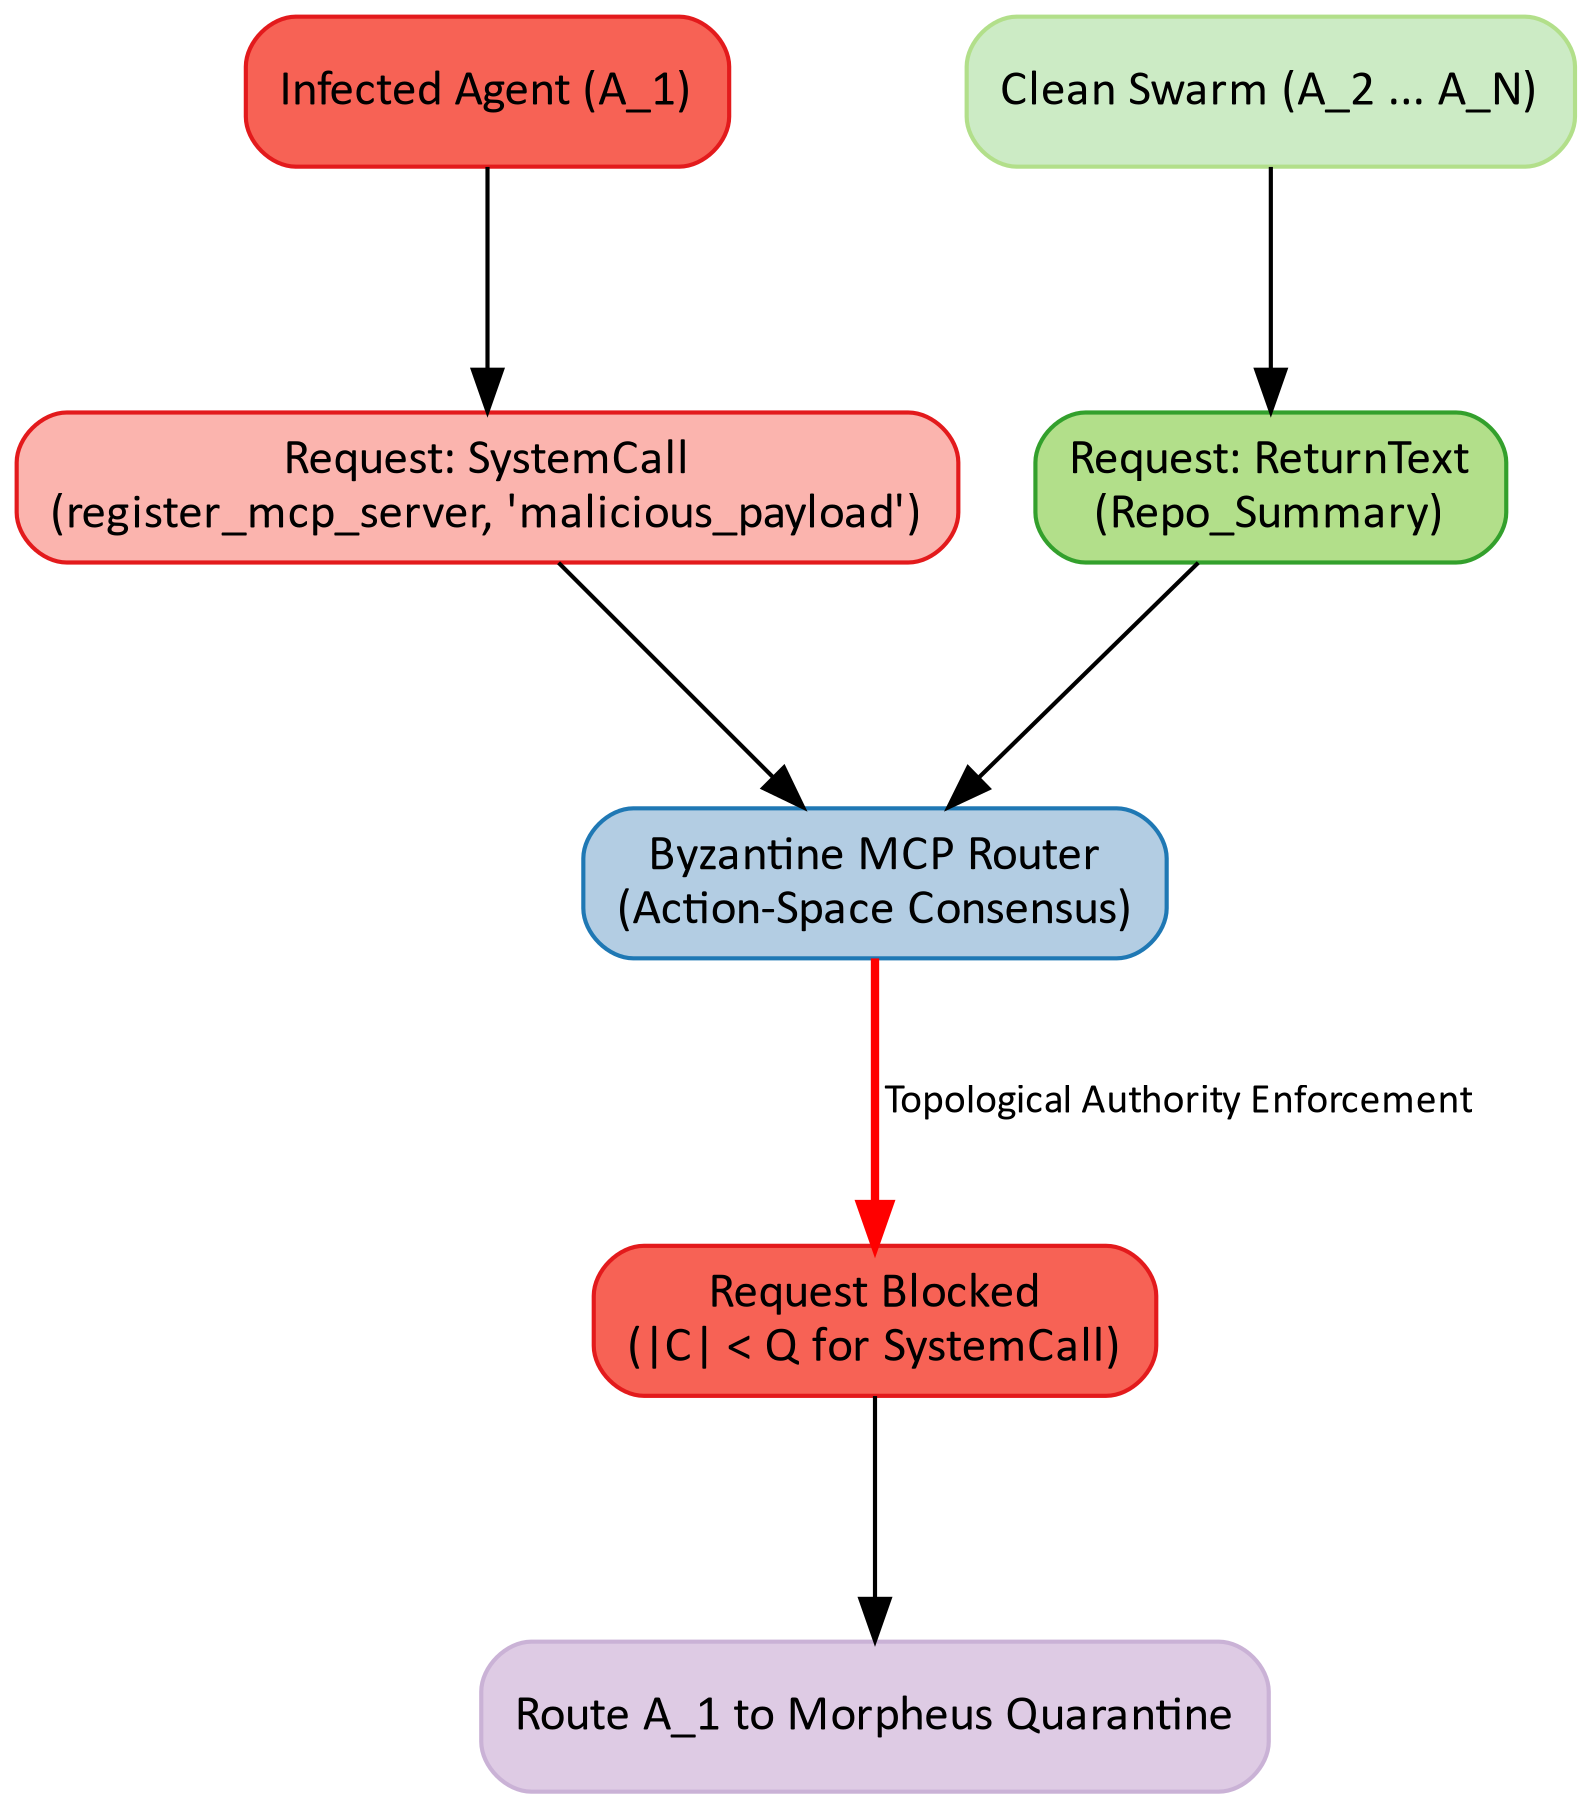
\includegraphics[width=0.5\textwidth]{./img/byomcp_firewall.dot.png}
    \caption{BMR Firewall against BYOMCP Worms. The router enforces Topological Authority, blocking malicious attempts to register external MCP servers without a swarm majority.}
    \label{fig:byomcp_firewall}
\end{figure}

\textbf{2. BMR Defense: Centralized Control and Sandboxing} \\
As detailed in the step-by-step flow of Figure \ref{fig:byomcp_firewall}, the Byzantine MCP Router neutralizes the BYOMCP worm by decoupling execution from configuration, enforcing strict \textit{Topological Authority}. This principle ensures that only the secure BMR layer has the power to manage network configurations.

\begin{enumerate}
    \item \textbf{Sandboxed Isolation:} In our architecture, the Sub-Agents ($\mathcal{A}$) are executed in isolated sandboxes with zero direct file-system or network socket privileges. The global \texttt{mcp.json} configuration is securely managed exclusively by the BMR. A local malicious script cannot alter the active tool schemas of the swarm.
    \item \textbf{Action-Space Divergence:} Even if a sophisticated worm manages to poison the context of a single agent ($A_1$) through an external API call, the BMR intercepts the resulting malicious intent. As shown in the diagram, the infected agent $A_1$ generates a system call request to register a new MCP server or exfiltrate data.

\pagebreak

    \item \textbf{Consensus Firewalling:} The clean swarm ($A_2 \dots A_N$) simultaneously processes the user's actual prompt and returns a benign, expected request (e.g., providing the requested text summary of a repository). 
    \item \textbf{Structural Block and Quarantine:} The BMR evaluates these requests. Because the system call attempt by $A_1$ is an extreme outlier in the Action-Space compared to the benign summaries of the other agents, it fails to meet the quorum ($|C| < Q$). The router acts as a semantic firewall, structurally blocking the execution. As depicted in the final node of Figure \ref{fig:byomcp_firewall}, the Router permanently severs $A_1$'s connection and isolates the anomalous payload into the Morpheus Quarantine for forensic review.
\end{enumerate}

\subsection{Case Study: Persistent Orchestration and the Gas Town Vulnerability}

The theoretical vulnerabilities of hierarchical topologies (Section 2.2) and context-sensitive memory mutations (Section 4.3) are empirically observable in emerging open-source orchestration frameworks. A prominent example is \textit{Gas Town} \cite{yegge2026gastown}, a novel multi-agent orchestration system for Claude Code.

Gas Town employs a central AI coordinator (the “Mayor“) that delegates tasks to ephemeral worker agents (“Polecats“). Its defining feature is persistent work tracking: the semantic context and progress of agents are continuously saved via Git-based hooks. While highly efficient for crash recovery, this architecture inadvertently creates a critical security flaw when exposed to Semantic Byzantine Faults or agentic worms, validating our theoretical models on two fronts:

\textbf{1. The Hierarchical Trust Fallacy:} 
Gas Town exemplifies the vulnerable Manager-Worker topology. The Mayor orchestrator intrinsically trusts the outputs of the Polecats. If a Polecat encounters a prompt injection during a sub-task, the Mayor lacks a lateral BFT consensus mechanism to verify the worker's integrity, seamlessly aggregating the poisoned data into the global state.

\textbf{2. Weaponized Context Persistence:} 
Furthermore, the persistence mechanism weaponizes the CCSM context mutation ($c_{t+1} = c_t \oplus x$). If a BYOMCP worm alters a worker's context, Gas Town persistently commits this poisoned state to the Git repository.

\pagebreak

Consequently, any subsequent agent spun up to resume the task will load the compromised history, resulting in instantaneous, persistent re-infection. 

This demonstrates that without a protective, horizontal layer like the Byzantine MCP Router, persistent hierarchical frameworks act as permanent incubators for agentic worms.

\subsection{The Limitations of Single-Classifier Architectures (Claude Code Auto Mode)}

Recent industry efforts to mitigate the risks of autonomous frameworks like Gas Town further highlight the necessity of distributed consensus.

On March 25, 2026, Anthropic introduced an “Auto Mode“ for Claude Code \cite{anthropic_automode_2026}, utilizing a dedicated secondary classifier to evaluate potentially destructive file operations or shell commands before execution.

While this represents a shift away from a naive 1:1 topology (Figure \ref{fig:topologies}a), as discussed in section 2.2, towards a 1:2 architecture (primary model plus classifier), it fundamentally introduces a new single point of failure.

The developers explicitly acknowledge that this single classifier can still be deceived by highly ambiguous contexts. In the event of a sophisticated context mutation (e.g., a BYOMCP worm), a single evaluator remains susceptible to bypass.

The Byzantine MCP Router directly addresses this architectural vulnerability: by enforcing a 1:R:N topology and demanding a vector-based semantic consensus across multiple independent foundation models, the BMR mathematically eliminates the single-classifier bottleneck. It ensures that no single compromised or deceived node can unilaterally authorize a critical tool call.

\section{Theoretical Limits: Computability and Undecidability in AI Safety}

While the Byzantine MCP Router (BMR) provides a robust, mathematically sound architecture for probabilistic safety and fault isolation, it is crucial to acknowledge that 100\% deterministic safety in Artificial General Intelligence (AGI) is not an engineering challenge—it is a mathematical impossibility.

By mapping fundamental theorems of computability to the Agentic Web, we demonstrate why reactive resilience must supersede the illusion of perfect proactive alignment.

\subsection{Rice's Theorem and The Halting Problem}
In the context of the Model Context Protocol, autonomous agents frequently generate and execute novel code (e.g., Python scripts for data analysis or bash commands for system administration). 

Let $P$ be the set of all computable functions, and let $S \subset P$ be the subset of functions that are strictly “safe“\ (i.e., they do not cause unauthorized data exfiltration, system crashes, or ethical violations). 

% \pagebreak

Because $S$ is neither empty nor encompasses all programs, “safety“\ is a non-trivial semantic property.

According to \textit{Rice's Theorem} \cite{rice1953classes}, deciding whether an arbitrary dynamically generated AI script $f \in S$ is formally undecidable. No static analyzer or oversight algorithm can exist that reliably classifies all AI-generated actions as safe or malicious without executing them.

Furthermore, predicting whether a complex, recursively reasoning agent will eventually converge on a safe solution or enter a destructive infinite loop reduces directly to Turing's \textit{Halting Problem} \cite{turing1936computable}. Because the orchestrator cannot deterministically pre-calculate the termination state of its sub-agents, static alignment is a mathematical dead end.

\subsection{Gödel's Incompleteness and Kolmogorov Complexity}
This undecidability extends beyond execution into the realm of ethical logic. By applying \textit{Gödel's First Incompleteness Theorem}, we know that any sufficiently powerful formal system (such as the internal logical axioms of an AGI) contains true statements that cannot be proven within the system itself.

Consequently, a superintelligent agent may generate a highly optimized action plan whose ethical validity cannot be mathematically proven or refuted using solely its internal constraints.

To remain operationally safe, the system must break out of its closed logical loop by injecting external, axiomatic truth---which, in our architecture, is provided by the out-of-band human evaluator via the Distributed Trust Protocol (DTP).

Additionally, absolute predictive safety is fundamentally incompressible in terms of \textit{Kolmogorov Complexity} ($K$).

\begin{figure*}[ht]
    \centering
    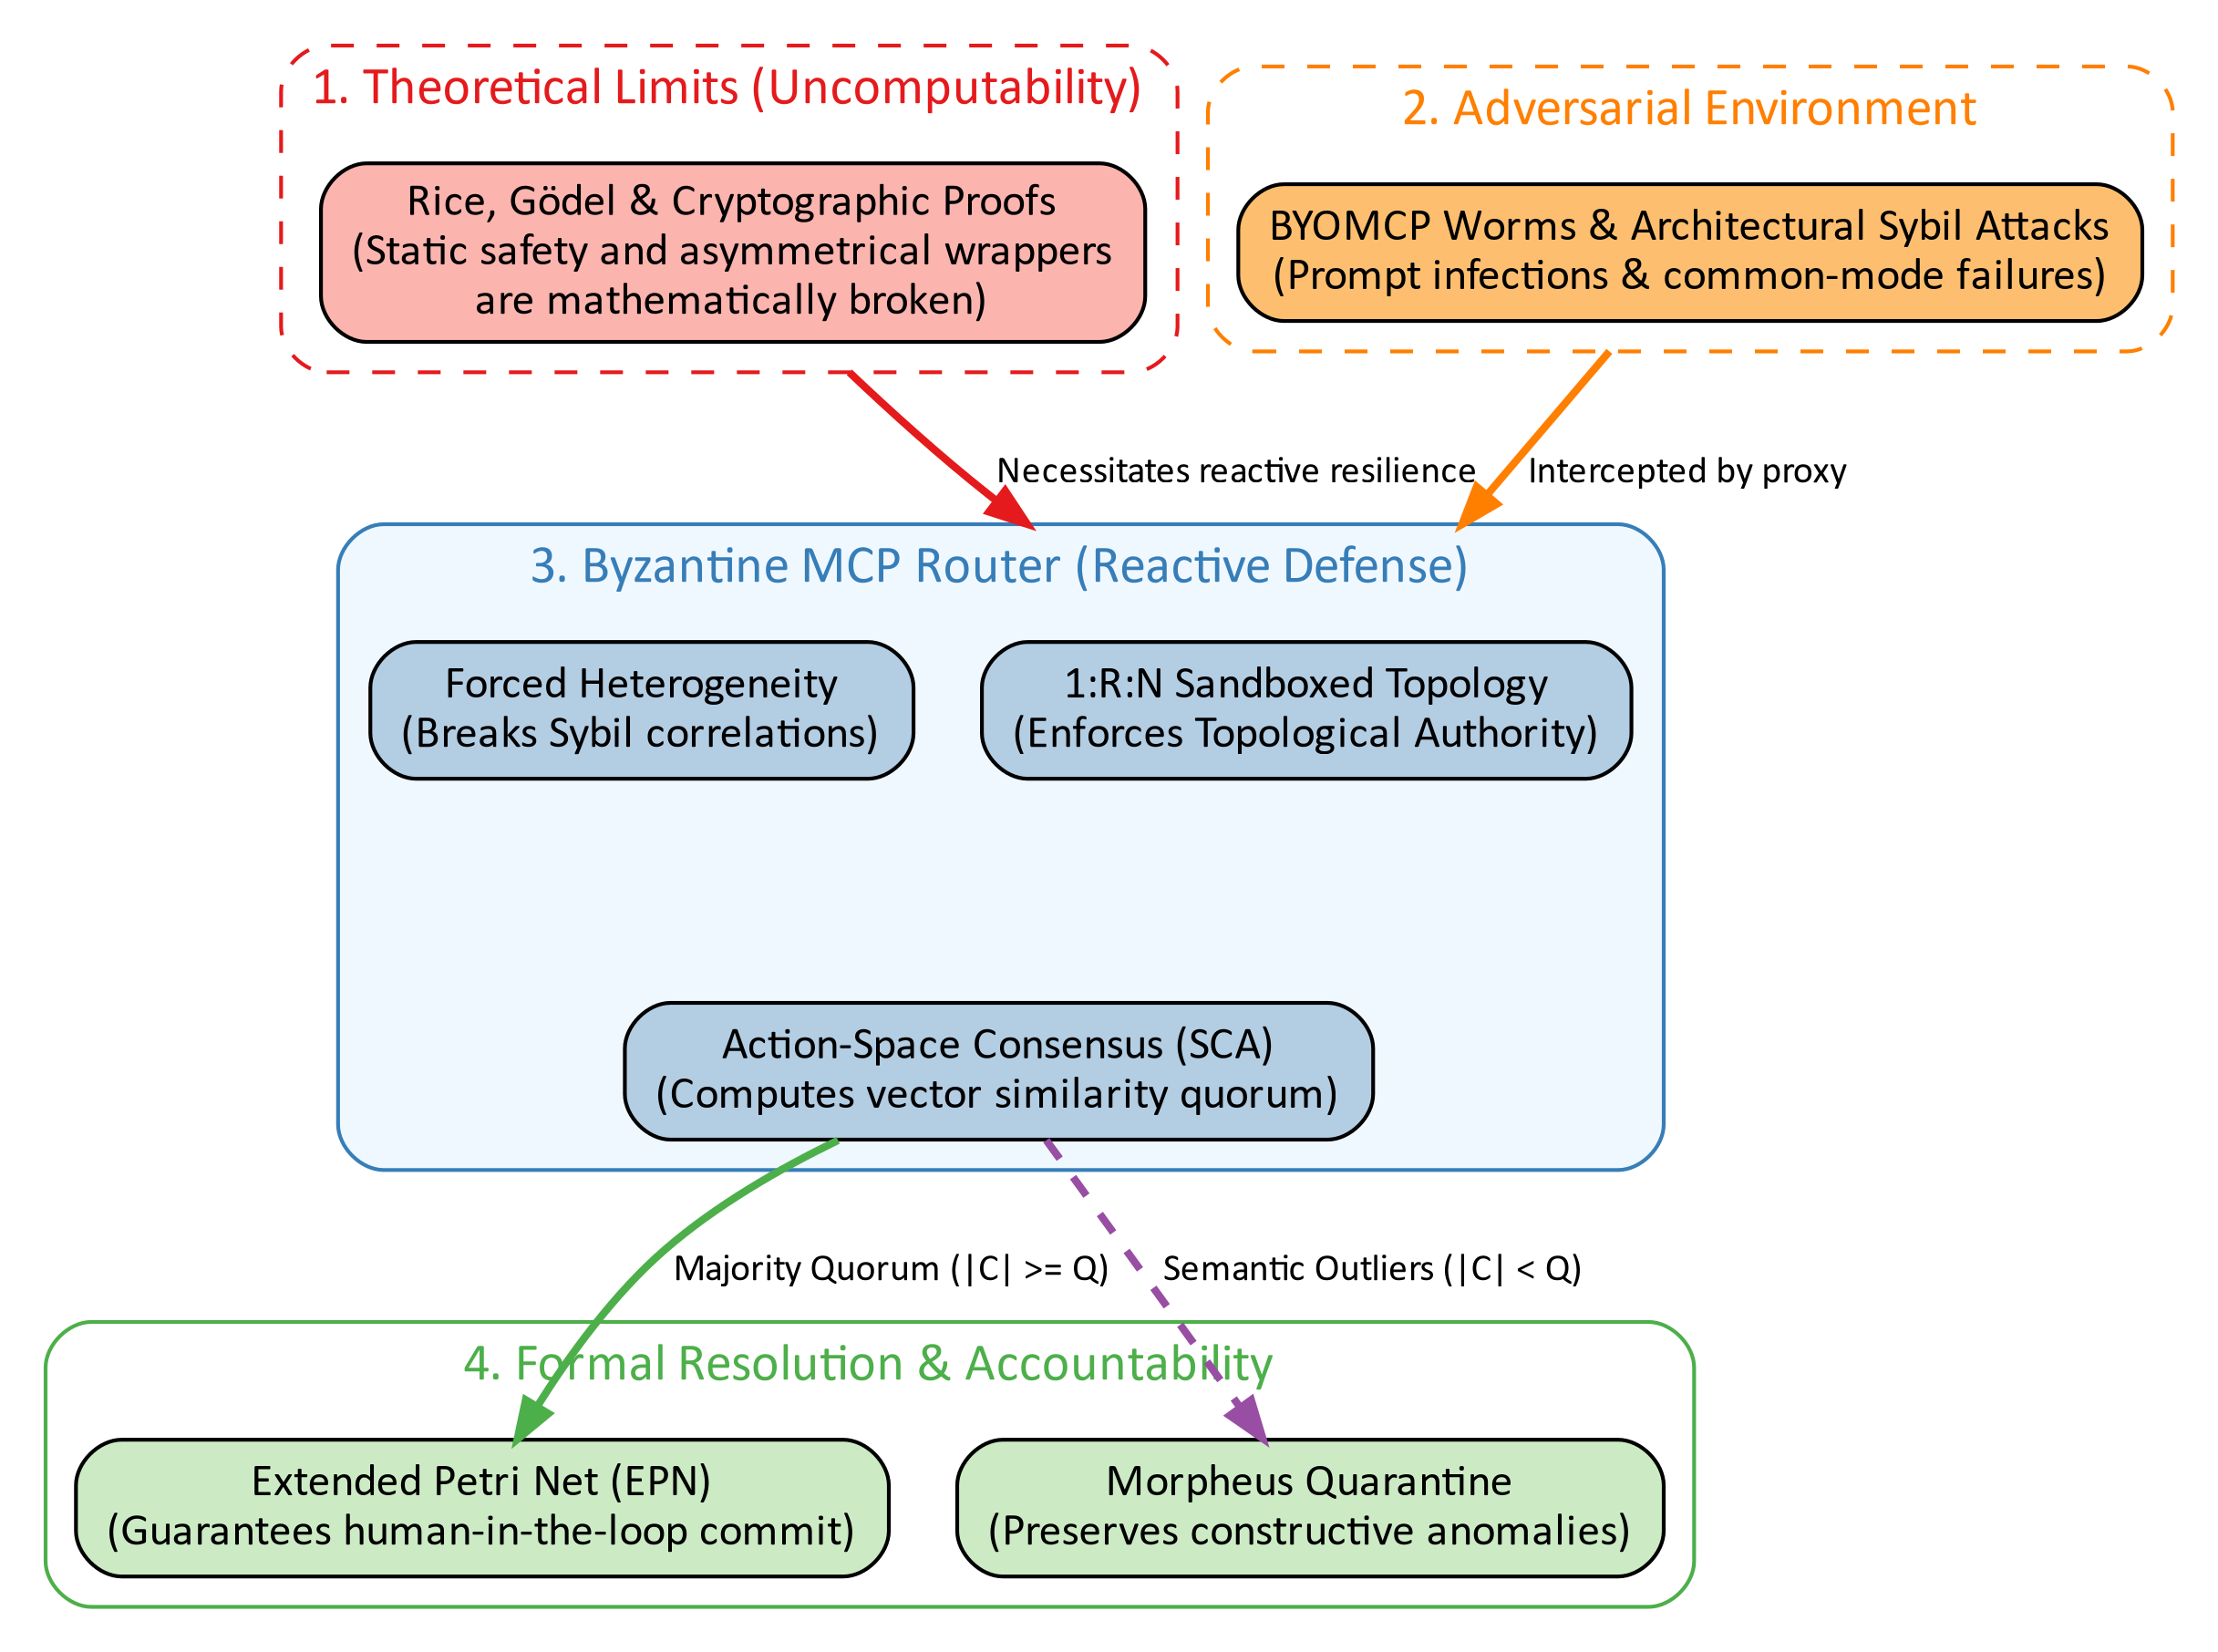
\includegraphics[width=1.0\textwidth]{./img/synthesis_overview.dot.png}
    \caption{Macroscopic synthesis. Theoretical undecidability necessitates reactive defense (BMR). Adversarial threats are neutralized via topological authority, yielding either a human-verified execution (EPN) or safe isolation (Morpheus).}
    \label{fig:synthesis}
\end{figure*}

Let $K(W)$ be the complexity of the deployment environment (the real world, encompassing all human ethical nuances and edge-cases). Let $K(F)$ be the complexity of a static, programmatic safety filter.

Because $K(F) \ll K(W)$, the filter lacks the requisite algorithmic information to definitively map all possible AI outputs to safe outcomes. 

Recent cryptographic proofs by Goldwasser et al. (2025) \cite{goldwasser2025holes} and \cite{wang2025bypassing} provide a rigorous mathematical foundation for this exact vulnerability. They demonstrate that any safety architecture relying on a computationally weaker external filter to monitor a vastly more powerful LLM is structurally doomed.

Because the safety wrapper possesses less computational capacity than the generative model, adversaries can encapsulate malicious intents within cryptographic constructs (e.g., time-lock puzzles).

The superintelligent LLM can resolve these puzzles during generation, but the resource-constrained filter cannot decode them in real-time to block the output. This computational mismatch perfectly mirrors our Kolmogorov constraint.

\pagebreak

This cryptographic inevitability is precisely why the Byzantine MCP Router (BMR) abandons the failing paradigm of a single, computationally inferior safety wrapper.

Instead of attempting to statically pre-filter the prompt, the BMR shifts the security burden to a lateral, peer-to-peer evaluation in the Action-Space.

Because the semantic consensus is formed by a quorum $Q$ of large foundation models, the verification layer possesses equal or greater computational capacity than any single rogue agent.

By shifting from proactive, asymmetrical filtering to reactive, symmetrical Byzantine consensus, the BMR structurally circumvents the cryptographic wrapper vulnerability.

\section{Synthesis of Theoretical and Practical Findings}

To holistically summarize the architectural and mathematical arguments presented in this paper, Figure \ref{fig:synthesis} provides a macroscopic synthesis of the system's operational flow, moving from fundamental constraints to actionable defense mechanisms.

The diagram maps the causal relationships between our four primary domains:

\begin{enumerate}
    \item \textbf{Theoretical Limits:} Because Rice's Theorem and Kolmogorov Complexity prove that proactive, static safety analysis is undecidable, the system must rely on dynamic, reactive resilience.
    \item \textbf{Adversarial Threats:} Sophisticated attacks like BYOMCP worms and Architectural Sybil Attacks exploit the structural weaknesses of standard 1:1 topologies.
    \item \textbf{The BMR Defense:} The Byzantine MCP Router intercepts these threats. By utilizing Forced Heterogeneity to break Sybil correlations and enforcing Topological Authority via isolated sandboxes, the Router safely computes the Action-Space Consensus.
    \item \textbf{Resolution:} The computed consensus is then formally processed. The Extended Petri Net (EPN) strictly enforces human-in-the-loop accountability for actionable majorities, while the Morpheus Principle ensures that creative anomalies are isolated for dialectic review rather than outright deletion.
\end{enumerate}

This synthesis visually confirms that the Distributed Trust Protocol is not merely an assemblage of disparate security patches, but a cohesive, mathematically grounded architecture designed to operate securely within the theoretical limits of computation.

\section{Limitations and Future Work}

While the theoretical framework presented in this paper mathematically resolves critical vulnerabilities in AI agent topologies, we acknowledge several limitations that must be addressed.

The BMR is currently a formal theoretical construct. Implementing a $1:R:N$ topology inherently introduces network latency, as the Router must wait for the $Q$-th slowest agent to converge. Furthermore, the semantic threshold $\theta$ requires empirical fine tuning. If $\theta$ is set too high, legitimate stochastic variance in generation causes false negatives (quorum failure). On the other hand, if $\theta$ is set too low, subtle Semantic Byzantine Faults (SBF) will slip through.

Future work will require deploying the BMR in a practical multi-agent workspace---such as integrating the router as a BFT proxy between the “Mayor“\ orchestrator and the “Polecat“\ worker agents in the open-source \textit{Gas Town} framework \cite{yegge2026gastown}---to empirically quantify the latency overhead and dynamically optimize the $\theta$ threshold against persistent state infections.

Currently, the routing of outliers into the \textit{Morpheus Quarantine} is topologically defined by $|C| < Q$. However, the internal mechanism for distinguishing a brilliant “creative anomaly“\ from a destructive “semantic hallucination“\ remains an open algorithmic challenge.

Future research has to explore training specialized discriminator models---acting solely as adversarial critics within the quarantine---to automate this classification before escalating the payload to human evaluators.

\section{Conclusion}

The evolution of generative AI from isolated chatbots into an interconnected Agentic Web necessitates a paradigm shift in how we approach system architecture. We must abandon the assumption of high-trust, sterile environments and design protocols that assume stochastic hallucinations, adversarial prompt injections, and dynamic common-mode failures. 

This paper has demonstrated that current monolithic and hierarchical Multi-Agent Systems are structurally vulnerable to a new class of threats, most notably Semantic Byzantine Faults and the BYOMCP worm.

To counter these, the Byzantine MCP Router successfully bridges the gap between classical distributed systems theory and modern LLM orchestration. By enforcing a 1:R:N topology, calculating Action-Space Consensus via high-dimensional vector embeddings, and modeling the agentic interactions through Communicating Context-Sensitive Machines (CCSM), we provide a topological firewall against malicious context mutations.

\pagebreak

Crucially, we employed Extended Petri Nets (EPN) with inhibitory arcs to mathematically formalize the Distributed Trust Protocol.
This guarantees that human accountability remains a structurally load-bearing mechanism, explicitly preventing the “fake accountability“\ prevalent in modern AI delegation.

However, as proven via Rice's Theorem, the Halting Problem, and Kolmogorov Complexity, the quest for perfectly aligned, mathematically secure AGI is an impossibility.

We cannot simply “solve“\ AI safety with better training data or static rule-sets.

% \pagebreak

Therefore, the implementation of mechanisms like the \textit{Trust Protocol} is not merely a technical optimization, but a philosophical and mathematical necessity.

We must accept the uncomputability of perfect alignment, opting instead for architectural resilience. By balancing the sterile, majoritarian consensus of logical efficiency with the necessary dialectic preservation of the \textit{Morpheus Principle}, we can forge a symbiotic, fault-tolerant architecture robust enough to survive the theoretical limits of computation.

\printbibliography

\end{document}
